%%%%%%%%%%%%%%%%%%%%%%%%%%%%%%%%%%%%%%%%%%%%%%%%%%%%%%%%%%%%%%%%%%%%%%%%%%%%
% USENIX Workshop on Large-Scale Exploits and Emergent Threats (LEET '08)
% April 2008
%%%%%%%%%%%%%%%%%%%%%%%%%%%%%%%%%%%%%%%%%%%%%%%%%%%%%%%%%%%%%%%%%%%%%%%%%%%%

%
% Some comment lines for separating sections of the latex file:
%

% High-level structure:
%===========================================================================
% Section:
%---------------------------------------------------------------------------
% Subsection:
%- - - - - - - - - - - - - - - - - - - - - - - - - - - - - - - - - - - - - -
% Subsubsection:
%. . . . . . . . . . . . . . . . . . . . . . . . . . . . . . . . . . . . . .
% Figure, etc.:
%o o o o o o o o o o o o o o o o o o o

\documentclass[letterpaper,twocolumn,11pt]{article}
\usepackage{usenix,epsfig}
\usepackage{boxedminipage}
%%%%%%%%%%%%%%%%%%%%%%%%%%%%%%%%%%%%%%%%%%%%%%%%%%%%%%%%%%%%%%%%%%%%%%%%%%%%%
%                                  PACKAGES                                 %
%%%%%%%%%%%%%%%%%%%%%%%%%%%%%%%%%%%%%%%%%%%%%%%%%%%%%%%%%%%%%%%%%%%%%%%%%%%%%

%\usepackage{epsfig}
\usepackage{amsmath}
\usepackage{amssymb}
\usepackage{amsthm}
\usepackage{amsfonts}
%\usepackage{pxfonts}
\usepackage{color}
\usepackage{subfigure}
%\usepackage[raggedright,normalsize,sf,SF,hang]{subfigure}
\usepackage{paralist}	% for compactenum etc
\usepackage{caption}
\usepackage{ifthen}
%\usepackage{substr}
%\renewcommand{\captionfont}{\sffamily}
%\usepackage[toc,page,title,titletoc]{appendix}
%\renewcommand{\restoreapp}{}
%\renewcommand{\appendixname}{Appendix}
\usepackage[noend]{algorithmic}
%\usepackage[nottoc]{tocbibind}

%%%%%%%%%%%%%%%%%%%%%%%%%%%%%%%%%%%%%%%%%%%%%%%%%%%%%%%%%%%%%%%%%%%%%%%%%%%%%
%                                  COMMANDS                                 %
%%%%%%%%%%%%%%%%%%%%%%%%%%%%%%%%%%%%%%%%%%%%%%%%%%%%%%%%%%%%%%%%%%%%%%%%%%%%%

\newcommand{\ignore}[1]{}
% An indexed term
\newcommand{\term}[1]{\index{#1}{\bfseries #1}}
% A term indexed differently from its name
%\newcommand{\termi}[2]{\index{#2}{\bfseries #1}}
\newcommand{\termi}[2]{{\bfseries #1}}
% A term that is not indexed
\newcommand{\termni}[1]{{\bfseries #1}}
\newcommand{\sumproduct}{sum--product}
%\newcommand{\sumproduct}{Shafer--Shenoy}
%\newcommand{\bk}{Boyen \& Koller (1998)}
%\newcommand{\bk}{BK}
%\newcommand{\tjtf}{TJTF}
\newcommand{\bk}{\textsc{b\&k98}}
%\newcommand{\tjtf}{TJTF}
\newcommand{\tjtf}{\textsc{tjtf}}
\newcommand{\dbn}{\textsc{dbn}}
\newcommand{\ttbn}{\textsc{2-tbn}}
\newcommand{\slat}{\textsc{slat}}
\newcommand{\rdpi}{\textsc{rdpi}}
\newcommand{\oca}{\textsc{oca}}

%%%%%%%%%%%%%%%%%%%%%%%%%%%%%%%%%%%%%%%%%%%%%%%%%%%%%%%%%%%%%%%%%%%%%%%%%%%%%
%                                 APPEARANCE                                %
%%%%%%%%%%%%%%%%%%%%%%%%%%%%%%%%%%%%%%%%%%%%%%%%%%%%%%%%%%%%%%%%%%%%%%%%%%%%%

% Change the font used for section headers to sans serif and make
% chapter headers centered.
%\usepackage{sectsty}
%\allsectionsfont{\sffamily}
%\chapterfont{\centering \sffamily}

%% \renewcommand\topfraction{.7}
%% \renewcommand\bottomfraction{.3}
%% \renewcommand\textfraction{.2}   
%% \renewcommand\floatpagefraction{.5}

%%%%%%%%%%%%%%%%%%%%%%%%%%%%%%%%%%%%%%%%%%%%%%%%%%%%%%%%%%%%%%%%%%%%%%%%%%%%%
%                                ENVIRONMENTS                               %
%%%%%%%%%%%%%%%%%%%%%%%%%%%%%%%%%%%%%%%%%%%%%%%%%%%%%%%%%%%%%%%%%%%%%%%%%%%%%

%\setcounter{secnumdepth}{5}
%\setcounter{tocdepth}{1}

\usepackage{framed}
\definecolor{gray}{cmyk}{0.05,0.05,0.05,0.05}
\newcommand{\shadecolor}{gray}
%\setlength{\fboxrule}{1pt}
%\setlength{\fboxsep}{1em}
%\newenvironment{highlight}[1][gray]%
%  {\vspace*{0.5\baselineskip} \begin{center}\begin{minipage}{0.85\textwidth}\renewcommand{\shadecolor}{#1}\begin{shaded}}%
%  {\end{shaded}\end{minipage}\end{center} \vspace*{0.5\baselineskip}}
\newenvironment{highlight}[1][white]%
  {\renewcommand{\shadecolor}{#1}\begin{shaded}}%
  {\end{shaded}}
\newenvironment{nohighlight}%
  {}%
  {}

\definecolor{pink}{cmyk}{0,0.1,0.1,0}

%\newenvironment{outline}{\begin{note} \begin{itemize}}{\end{itemize} \end{note}}
%\newcommand{\commentout}[1]{}

% Definitions.
%\newtheoremstyle{mythmstyle}% name
%  {0pt}%      Space above
%  {0pt}%      Space below
%  {}%         Body font
%  {}%         Indent amount (empty = no indent, \parindent = para indent)
%  {\bfseries}%Thm head font
%  {.}%        Punctuation after thm head
%  { }%        Space after thm head: " " = normal interword space;
%        %       \newline = linebreak
%  {}%         Thm head spec (can be left empty, meaning `normal')
%\theoremstyle{mythmstyle}

\newtheorem{theorem}{Theorem}%[chapter]
\newtheorem{lemma}{Lemma}%[chapter]
\newtheorem{corollary}{Corollary}%[chapter]
\newtheorem{property}{Property}%[chapter]
\newtheorem{definition}{Definition}%[chapter]
\newtheorem{example}{Example}%[chapter]
\newtheorem{algorithm}{Algorithm}%[chapter]

%\newtheorem{thm}{Theorem}%[chapter]
%\newtheorem{lem}{Lemma}%[chapter]
%\newtheorem{corr}{Corollary}%[chapter]
%\newtheorem{prop}{Property}%[chapter]
%\newtheorem{defn}{Definition}%[chapter]
%\newtheorem{exam}{Example}%[chapter]
%\newtheorem{alg}{Algorithm}%[chapter]

%\newenvironment{algorithm}[1]{\begin{nohighlight} \begin{alg} \mbox{\emph{#1}}}{\end{alg} \end{nohighlight}}
%\newenvironment{example}{\begin{nohighlight} \begin{exam}}{\end{exam} \end{nohighlight}}
%\newenvironment{definition}{\begin{nohighlight} \begin{defn}}{\end{defn} \end{nohighlight}}
%\newenvironment{theorem}{\begin{nohighlight} \begin{thm}}{\end{thm} \end{nohighlight}}
%\newenvironment{lemma}{\begin{nohighlight} \begin{lem}}{\end{lem} \end{nohighlight}}
%\newenvironment{corollary}{\begin{highlight} \begin{corr}}{\end{corr} \end{nohighlight}}
%\newenvironment{property}{\begin{highlight} \begin{prop}}{\end{prop} \end{nohighlight}}

%%%%%%%%%%%%%%%%%%%%%%%%%%%%%%%%%%%%%%%%%%%%%%%%%%%%%%%%%%%%%%%%%%%%%%%%%%%%%
%                                  NOTATION                                 %
%%%%%%%%%%%%%%%%%%%%%%%%%%%%%%%%%%%%%%%%%%%%%%%%%%%%%%%%%%%%%%%%%%%%%%%%%%%%%

%%%%%%%%%%%%%%%%%%%%%%%%%%%%%%%%%% General %%%%%%%%%%%%%%%%%%%%%%%%%%%%%%%%%% 

\providecommand{\abs}[1]{\ensuremath{\lvert#1\rvert}}
\providecommand{\norm}[1]{\ensuremath{\lVert#1\rVert}}
\providecommand{\bignorm}[1]{\ensuremath{\bigl\lVert#1\bigr\rVert}}
\providecommand{\Bignorm}[1]{\ensuremath{\Bigl\lVert#1\Bigr\rVert}}
%\newcommand{\norm}[1]{\ensuremath{||#1||}}
%\newcommand{\implies}{\ensuremath{\Longrightarrow}}
%\newcommand{\iff}{\ensuremath{\Longleftrightarrow}}
\newcommand{\bzero}{\ensuremath{\boldsymbol{0}}}
\newcommand{\bone}{\ensuremath{\boldsymbol{1}}}
\newcommand{\df}[1]{\ensuremath{\textrm{d}#1}}
\newcommand{\tr}[1]{\ensuremath{\textrm{trace}(#1)}}
\newcommand{\transpose}{\ensuremath{\top}}
\newcommand{\reals}{\ensuremath{\mathbb{R}}}
\newcommand{\nonnegreals}{\ensuremath{\mathbb{R}^+}}
\newcommand{\nonnegints}{\ensuremath{\mathbb{Z}^+}}
%\newcommand{\defeq}[0]{\ensuremath{\stackrel{\triangle}{=}}}
\newcommand{\defeq}{\triangleq}
\newcommand{\setdiff}{\ensuremath{-}}
\newcommand{\indicator}[1]{\ensuremath{\boldsymbol{1}\{ #1 \}}}
\newcommand{\set}[1]{\ensuremath{\left\{ #1 \right\}}}
\newcommand{\E}[1]{\ensuremath{\mathbb{E}[{#1}]}}
\newcommand{\Cov}[1]{\ensuremath{\textrm{Cov}[{#1}]}}
\newcommand{\kl}[2]{\ensuremath{D(#1 \, \| \, #2)}}
\newcommand{\opt}{\ensuremath{\ast}}
\DeclareMathOperator*{\argmax}{arg max}
\DeclareMathOperator*{\argmin}{arg min}
\newcommand{\card}[1]{\ensuremath{|#1|}}
\newcommand{\scope}[1]{\ensuremath{\textrm{Scope}[{#1}]}}
\newcommand{\assign}{\leftarrow}
%%%%%%%%%%%%%%%%%%%%%%%%%%%%%%%%% Sets %%%%%%%%%%%%%%%%%%%%%%%%%%%%%%%%%%%%%%

%% The arguments of a factor: \args{node}
\newcommand{\args}[1]{{\ensuremath \iset{A}_{#1}}}

%%%%%%%%%%%%%%%%%%%%%%%%%%%%%%%%% Processes %%%%%%%%%%%%%%%%%%%%%%%%%%%%%%%%% 

%% A stochastic process: \proc[letter]
\newcommand{\proc}[1][x]{{\ensuremath \mathbf{\uppercase{#1}}}}
% A process index: \ind{letter}
\newcommand{\ind}[1]{{\ensuremath{\lowercase{#1}}}}
\newcommand{\varind}[1]{{\ensuremath{\textsc{\lowercase{#1}}}}}
% Three generic indices.
\newcommand{\inda}{\ind{a}}
\newcommand{\indb}{\ind{b}}
\newcommand{\indc}{\ind{c}}
\newcommand{\indd}{\ind{d}}
\newcommand{\inde}{\ind{e}}
\newcommand{\indf}{\ind{f}}
\newcommand{\indg}{\ind{g}}
\newcommand{\indh}{\ind{h}}
\newcommand{\indi}{\ind{i}}
\newcommand{\indj}{\ind{j}}
\newcommand{\indk}{\ind{k}}

%% A process variable: \rv[letter]{index}
\newcommand{\rv}[2][x]{{\ensuremath \uppercase{#1}_{#2}}}
%% A process value: \rval[letter]{index}
%\newcommand{\rval}[2][x]{{\ensuremath \lowercase{#1}_{#2}}}
%% A fixed process value: \frval[letter]{index}
\newcommand{\frval}[2][x]{{\ensuremath \overline{\lowercase{#1}}_{#2}}}
%% A subprocess index set: \iset{letter}
\newcommand{\iset}[1]{{\ensuremath{\uppercase{#1}}}}
%% The index set of the global process.
\newcommand{\univ}{\iset{V}}
%% The index set of the query variables: \query[\node]
\newcommand{\query}[1]{\ensuremath{\iset{Q}_{#1}}}
%% The index set of the evidence variables.
\newcommand{\evidence}[1]{\iset{E}_{#1}}
%% The index set of the parent variables of a variable: \parents{index}.
\newcommand{\parents}[1]{\textrm{Pa}[{#1}]}
\newcommand{\pa}[1]{\parents{#1}}

%% The index set of the parent variables of a variable: \parents{index}.
%\newcommand{\parents}[1]{\ensuremath{\textbf{Pa}[{#1}]}}
%\newcommand{\pa}[1]{\parents{#1}}

%% Three generic index sets.
\newcommand{\iseta}{\iset{S}}
\newcommand{\isetb}{\iset{T}}
\newcommand{\isetc}{\iset{U}}
\newcommand{\isetd}{\iset{R}}
%% A stochastic subprocess: \subproc[letter]{indexset}
\newcommand{\subproc}[2][x]{{\ensuremath \mathbf{\uppercase{#1}}_{#2}}}
%% The index set of discrete variables.
\newcommand{\discrete}{\iset{D}}
%% The index set of continuous variables.
\newcommand{\continuous}{\iset{C}}

%% Annotation
\newcommand{\annot}[2]{%
\def\empty{}%
\def\targ{#2}%
\ifx\targ\empty \ensuremath{#1}%
\else \ensuremath{{#1}^{#2}}%
\fi}

%% Double annotation
\newcommand{\dannot}[3]{%
\def\empty{}%
\def\targ{#2}%
\ifx\targ\empty \ensuremath{#1_{#3}}%
\else \ensuremath{{#1}^{#2}_{#3}}%
\fi}

% Time indexing, e.g., \ti{\rvals{x}}{t}
% The following definition typesets the time index only if it is specified
\newcommand{\ti}[2]{
  \def\empty{}
  \def\targ{#2}
  \ifx\targ\empty
    \ensuremath{#1}
  \else
    \ensuremath{{#1}^{(#2)}}
  \fi}
% Component indexing, e.g., \ci{\rvals{x}}{i}
\newcommand{\ci}[2]{\ensuremath{{#1}_{#2}}}
% Both time and component indexing, e.g., \tci{\rvals{x}}{t}{i}
\newcommand{\tci}[3]{
  \def\empty{}
  \def\targ{#2}
  \ifx\targ\empty
    \ensuremath{{#1}_{#3}}
  \else
    \ensuremath{{#1}_{#3}^{(#2)}}
  \fi}
% A time index range: \range{t}{t'}
\newcommand{\range}[2]{\ensuremath{{#1}:{#2}}}

% A random variable
\newcommand{\rvar}[1]{\ensuremath{\MakeUppercase{#1}}}
% A value of a random variable
\newcommand{\rval}[1]{\ensuremath{\MakeLowercase{#1}}}
% A set/vector of random variables
\newcommand{\rvars}[1]{\ensuremath{\MakeUppercase{{\bf #1}}}}
% A value of a set/vector of random variables
\newcommand{\rvals}[1]{\ensuremath{\MakeLowercase{{\bf #1}}}}

% Some common combinations of variables/values and indices
\newcommand{\rvalti}[2]{\ensuremath{\ti{\rval{#1}}{#2}}}
\newcommand{\rvarti}[2]{\ensuremath{\ti{\rvar{#1}}{#2}}}
\newcommand{\rvalci}[2]{\ensuremath{\ci{\rval{#1}}{#2}}}
\newcommand{\rvarci}[2]{\ensuremath{\ci{\rvar{#1}}{#2}}}
\newcommand{\rvalsti}[2]{\ensuremath{\ti{\rvals{#1}}{#2}}}
\newcommand{\rvarsti}[2]{\ensuremath{\ti{\rvars{#1}}{#2}}}
\newcommand{\rvalsci}[2]{\ensuremath{\ci{\rvals{#1}}{#2}}}
\newcommand{\rvarsci}[2]{\ensuremath{\ci{\rvars{#1}}{#2}}}
\newcommand{\rvaltci}[3]{\ensuremath{\tci{\rval{#1}}{#2}{#3}}}
\newcommand{\rvartci}[3]{\ensuremath{\tci{\rvar{#1}}{#2}{#3}}}
\newcommand{\rvalstci}[3]{\ensuremath{\tci{\rvals{#1}}{#2}{#3}}}
\newcommand{\rvarstci}[3]{\ensuremath{\tci{\rvars{#1}}{#2}{#3}}}

%%%%%%%%%%%%%%%%%%%%%%%%%%%%%%%%% Densities %%%%%%%%%%%%%%%%%%%%%%%%%%%%%%%%% 

% A generic function: \function{symbol}{annot}{args}
% Leaves out the arguments if the args are empty
\newcommand \function[3]{\ensuremath{
  \def\args{#3}
  \def\empty{}
  \ifx\args\empty
    {#1}_{#2}
  \else
    {#1}_{#2}(#3)
  \fi}}
%% Probability
%\newcommand{\probability}{\ensuremath{\wp}}
%% Given
\newcommand{\given}{{\ensuremath \vert}}
%% Probability
\newcommand{\pr}[1]{\ensuremath{\textrm{Pr}\left[#1\right]}}
%% Conditional probability
\newcommand{\cpr}[2]{\ensuremath{\textrm{Pr}\left[#1 \,\given\, #2\right]}}
%% Density: \p
\newcommand{\p}[2][]{\function{\textsl{p}}{#1}{#2}}
%% Conditional density: \cp{vars}{vars}
\newcommand{\cp}[3][]{\p[#1]{#2 \given #3}}
%% Approximate density: \ap
\newcommand{\ap}[2][]{\function{\tilde{\textsl{p}}}{#1}{#2}}
%% Approximate conditional density: \acp{vars}{vars}
\newcommand{\acp}[3][]{\ap[#1]{#2 \given #3}}
%% Other density: \q
\newcommand{\q}[2][]{\function{\textsl{q}}{#1}{#2}}
%% Empirical distribution: \empp
\newcommand{\empp}[2][]{\function{\hat{\textsl{p}}}{#1}{#2}}
%% Counts (a special case of an empirical distribution):
\newcommand{\counts}[1]{\ensuremath{\text{Count}\left[{#1}\right]}}

%% Independence statement: \condind{indexset1}{indexset2}{indexset3}
%\newcommand{\indep}{{\bot\negthickspace\negthickspace\bot}
\newcommand{\indep}{{\,\bot\,}}
\newcommand{\margind}[2]{{\ensuremath #1 \, \indep \, #2}}
\newcommand{\condind}[3]{{\ensuremath #1 \, \indep \, #2 \, \vert \, #3}}

% Independence relations: \indeprel[annotation]{graph_or_distribution}
\newcommand{\indeprel}[1]{\ensuremath{\cal{I}(#1)}}

%% Markov graph
\newcommand{\markov}[1][{}]{{\ensuremath G_{#1}}}

%%%%%%%%%%%%%%%%%%%%%%%%%%%%%%%%%%% Trees %%%%%%%%%%%%%%%%%%%%%%%%%%%%%%%%%%% 

%% A graph
\newcommand{\graph}[1][{}]{\annot{G}{#1}}
%% A tree: \tree[annotation]
\newcommand{\tree}[1][{}]{\annot{T}{#1}}
% A node: \node{letter} (deprecated)
\newcommand{\node}[1]{{\ensuremath{\lowercase{#1}}}}
% Two generic nodes (deprecated)
\newcommand{\n}[1][]{\node{n}_{#1}}
\newcommand{\m}{\node{m}}
%\newcommand{\l}{\ell}
% Some more generic nodes (deprecated)
\newcommand{\na}{\node{i}}
\newcommand{\nb}{\node{j}}
\newcommand{\nc}{\node{k}}
\newcommand{\nd}{\node{h}}
\newcommand{\nf}{\node{\ell}}
\newcommand{\nh}{\node{f}}
\newcommand{\nj}{\node{g}}
\newcommand{\nm}{\node{m}}
\newcommand{\nn}{\node{n}}
%% The node set of a tree
\newcommand{\nodes}[1][\tree]{\ensuremath{N_{#1}}}
%% The edges of a tree (should be clear from context)
\newcommand{\edges}[1][\tree]{\ensuremath{E_{#1}}}
%% The directed edges of a tree (deprecated)
\newcommand{\dedges}[1][\tree]{\ensuremath{\vec{E}_{#1}}}
%% The undirected edges of a tree (deprecated)
\newcommand{\uedges}[1][\tree]{\ensuremath{E_{#1}}}
%% Directed edge: \dedge{from}{to}
\newcommand{\dedge}[2]{\ensuremath{(#1, #2)}}
%% Undirected edge: \uedge{node1}{node2}
\newcommand{\uedge}[2]{\ensuremath{\{#1, #2\}}}
%% Neighbors of a node: \nbr{node}
\newcommand{\nbr}[2][\tree]{\ensuremath{\nodes[{#1}](#2)}}
%% Descendants under an edge: \desc{from}{to}
\newcommand{\desc}[2]{\ensuremath{D\dedge{#1}{#2}}}
%% Rooted tree: \rootedtree
\newcommand{\rootedtree}{\ensuremath{\vec{T}}}
%% Node set: \nset[accent]{index}
\newcommand{\nset}[1][]{\ensuremath{M_{#1}}}
%% An upstream neighbor: \upnbr{node}
\newcommand{\upnbr}[1]{\ensuremath{up(#1)}}
%% Root node
\newcommand{\nroot}[0]{r}
%% Edge weight
\newcommand{\eweight}[2]{\ensuremath{w_{#1,#2}}}
%% Line representing an edge
\newcommand{\uedgel}[0]{\longleftrightarrow}


%%%%%%%%%%%%%%%%%%%%%%%%%%%%%%%%% Assignments %%%%%%%%%%%%%%%%%%%%%%%%%%%%%%% 

% A dummy assignment to a set of variables: \das{indexset}
\newcommand{\as}[2][x]{{\ensuremath{\textbf{\lowercase{#1}}_{#2}}}}
% A fixed assignment to a set of variables: \fas{indexset}
\newcommand{\fas}[2][x]{{\ensuremath{\overline{\textbf{\lowercase{#1}}}_{#2}}}}
% The evidence assignment.
%\newcommand{\obs}[1][]{\fas{\evidence[#1]}}
% The restriction of an assignment to a subset of
% variables: \restr{assignment}{varset}
\newcommand{\restr}[2]{{\ensuremath{{#1}:{#2}}}}
% The union of two disjoint assignments: \union{assignment1}{assignment2}
\newcommand{\union}[2]{{\ensuremath{#1 \cup #2}}}

%%%%%%%%%%%%%%%%%%%%%%%%%%%%% Variable elimination %%%%%%%%%%%%%%%%%%%%%%%%%%

%% An elimination factor: \elim[\pre|\post]{var}
\newcommand{\pre}{}
\newcommand{\post}{{\ensuremath \ast}}
\newcommand{\elim}[2][\pre]{{\ensuremath \xi^{#1}_{#2}}}
%% An elimination clique: \eclique{var}
\newcommand{\eclique}[1]{{\ensuremath \iset{E}_{#1}}}

%%%%%%%%%%%%%%%%%%%%%%%%%%%%%%%% Clique trees %%%%%%%%%%%%%%%%%%%%%%%%%%%%%%%

% The following typesetting could be improved...

%% A clique tree.
%\newcommand{\ct}{{\ensuremath \mathfrak{T}}}
%% A set of cliques: \cliques[annotation]
\newcommand{\cliques}[1][{}]{\annot{\mathbf{C}}{#1}}
\newcommand{\subcliques}[1]{\ensuremath{\cliques_{#1}}}
%% The clique of a node: \clique[annotation]{node}
\newcommand{\clique}[2][{}]{\dannot{C}{#1}{#2}}
%% The clique of a node, indexed by time: \cliqueti[time]{node}
%\newcommand{\cliqueti}[2][{}]{\ensuremath{\rvarstci{C}{#1}{#2}}}
%% A separator between a pair of nodes: \sep[annotation]{node1}{node2}
\newcommand{\sep}[3][{}]{\dannot{S}{#1}{#2,#3}}
%% A separator between a pair of nodes: \septi[time]{node1}{node2}
%\newcommand{\septi}[3][{}]{\ensuremath{\rvarstci{S}{#1}{#2,#3}}}
%% The elements reachable via an edge: \reach[annotation]{node1}{node2}
\newcommand{\reach}[3][]{\ensuremath{R^{#1}_{#2,#3}}}
%% The elements reachable exclusively via an edge: \ereach{node1}{node2}
\newcommand{\ereach}[2]{\reach[\ast]{#1}{#2}}
%% Cliques in the message between two nodes
%\newcommand{\mcliques}[2]{{\ensuremath \mathbf{C}_{#1 \rightarrow #2}}}

%%%%%%%%%%%%%%%%%%%%%%%%% Clique tree parameterization %%%%%%%%%%%%%%%%%%%%%%

%% The factors of a clique tree: \factors[annot]
\newcommand{\factors}[1][{}]{{\ensuremath \boldsymbol{\psi}^{#1}}}
%% A factor of a clique tree: \factor[node]
\newcommand{\factor}[1]{\ensuremath{\psi_{#1}}}
%% Another arbitrary factor: \otherfactor[marker]
\newcommand{\otherfactor}[1][{}]{{\ensuremath \gamma_{#1}}}

%%%%%%%%%%%%%%%%%%%%%%%%%%%%%%%%% Sum-product %%%%%%%%%%%%%%%%%%%%%%%%%%%%%%%

%% The message from one node to another: \msg[accent]{from}{to}
\newcommand{\msg}[3][]{\dannot{\mu}{#1}{#2, #3}}  % \rightarrow
\newcommand{\msgs}[1][]{\annot{{\boldsymbol \mu}}{#1}}
%% The node belief of a node: \nbel[accent]{node}
\newcommand{\nbel}[2][{}]{\ensuremath{\beta_{#2}^{#1}}}
%% The edge belief of an edge: \ebel[accent]{node1}{node2}
\newcommand{\ebel}[3][{}]{\ensuremath{\beta_{#2,#3}^{#1}}}

%%%%%%%%%%%%%%%%%%%%%%%%% Asynchronous message passing %%%%%%%%%%%%%%%%%%%%%%

%% A sum-product charge (possibly accented)
\newcommand{\spchg}[1][{}]{{\ensuremath \boldsymbol{\eta}^{#1}}}
%% An accent to indicate an updated value
\newcommand{\updated}{{\ensuremath \star}}
%% The sum-product charge on a directed edge (possibly
%% accented): \spchge[accent]{node1}{node2}
\newcommand{\spchge}[3][{}]{{\ensuremath \eta_{\dedge{#2}{#3}}^{#1}}}

%%%%%%%%%%%%%%%%%%%%%%%%%%%%%%%%%%% Hugin %%%%%%%%%%%%%%%%%%%%%%%%%%%%%%%%%%%

%% A Hugin charge (possibly accented)
\newcommand{\hchg}[1][{}]{{\ensuremath \boldsymbol{\phi}^{#1}}}
%% A Hugin node charge (possibly accented): \hchgn[accent]{node}
\newcommand{\hchgn}[2][{}]{{\ensuremath \phi_{#2}^{#1}}}
%% A Hugin edge charge (possibly accented): \hchge[accent]{node1}{node2}
\newcommand{\hchge}[3][{}]{{\ensuremath \phi_{\uedge{#2}{#3}}^{#1}}}
%% The contraction of a Hugin charge: \contr[charge]
\newcommand{\contr}[1][\hchg]{{\ensuremath \chi_{#1}}}

%%%%%%%%%%%%%%%%%%%%%%%%%%% Multivariate Gaussians %%%%%%%%%%%%%%%%%%%%%%%%%%

%% A random vector: \rvec{indexes}
\newcommand{\rvec}[2][x]{\ensuremath{\vec{\mathbf{\uppercase{#1}}}_{#2}}}
%% A subvector of a random vector: \subrvec{indexes}
%\newcommand{\subrvec}[2][x]{{\ensuremath \rvec[#1]_{#2}}}
% A vector value: \asv{letter}
\newcommand{\asv}[2][x]{\ensuremath{\vec{\mathbf{\lowercase{#1}}}_{#2}}}

%% Moment form Gaussians
% The mean vector (subscripted, possibly annotated [TODO])
\newcommand{\mean}[1]{\ensuremath{\mu_{#1}}}
% The covariance matrix (subscripted)
\newcommand{\cov}[1]{\ensuremath{\Sigma_{#1}}}
% A moment-parameterized Gaussian: \momentg{mean}{cov}
\newcommand{\momentg}[2]{\ensuremath{{\mathcal N}\left(#1, #2\right)}}
% Approximated mean vector (subscripted) 
\newcommand{\amean}[1]{\tilde{\mu}_{#1}}
% Approximated covariance matrix (subscripted)
\newcommand{\acov}[1]{\tilde{\Sigma}_{#1}}

%% Canonical form Gaussians
% The information vector (subscripted)
\newcommand{\ivec}[1]{\eta_{#1}}
% The information matrix (subscripted)
\newcommand{\imat}[1]{\Lambda_{#1}}
% A canonical-parameterized Gaussian: \canonicalg{ivec}{imat}
\newcommand{\canonicalg}[2]{\ensuremath{{\mathcal N}^{-1}\left(#1, #2\right)}}
% The information vector (subscripted)
\newcommand{\aivec}[1]{\tilde{\eta}_{#1}}
% The information matrix (subscripted)
\newcommand{\aimat}[1]{\tilde{\Lambda}_{#1}}

% A Gaussian factor: \gfactor{subrvec}{ivec}{imat}
\newcommand{\gfactor}[3]{\ensuremath{{\mathcal G}\left(#1; #2, #3\right)}}

%%%%%%%%%%%%%%%%%%%%%%%%% Dynamic Bayesian networks %%%%%%%%%%%%%%%%%%%%%%%%

% Indexing an attribute by time: \ti{index}{time}
%\newcommand{\ti}[2]{{\ensuremath {#1}(#2)}}
% Indexing an attribute set by time: \tis{indexset}{time}
%\newcommand{\tis}[2]{{\ensuremath {#1}(#2)}}
% The states of a DBN
%\newcommand{\states}{\iset{w}}
% A time index range: \trange{t}{t'}
%\newcommand{\trange}[2]{{\ensuremath {#1}:{#2}}}

% The state variables in a DBN: \statevars[time]
\newcommand{\State}[2][{}]{\rvarstci{x}{#1}{#2}}
% Assignments to state variables: \statevals[time]
\newcommand{\state}[2][{}]{\rvalstci{x}{#1}{#2}}
% A single state variable: \statevar[time]{index}
\newcommand{\sState}[2][{}]{\rvartci{x}{#1}{#2}}
% Assignment to a single state variable: \stateval[time]{index}
\newcommand{\sstate}[2][{}]{\rvaltci{x}{#1}{#2}}

% The variable representing a class
\newcommand{\Class}[2][{}]{\rvarstci{y}{#1}{#2}}
% Assignments to state variables: \statevals[time]
\newcommand{\class}[2][{}]{\rvalstci{y}{#1}{#2}}

% The observations: \obsvars[time]
\newcommand{\Obs}[2][{}]{\rvarstci{z}{#1}{#2}}
% Values of observation variables: \obsvals[time]
\newcommand{\obs}[2][{}]{\rvalstci{z}{#1}{#2}}
\newcommand{\fobs}[2][{}]{\rvalstci{\underline{z}}{#1}{#2}}
% An observation variable in a DBN: \obsvar[time]{index}
\newcommand{\sObs}[2][{}]{\rvartci{z}{#1}{#2}}
% Value of an observation variable
\newcommand{\sobs}[2][{}]{\rvaltci{z}{#1}{#2}}
\newcommand{\sfobs}[2][{}]{\rvaltci{\underline{z}}{#1}{#2}}

%%%%%%%%%%%%%%%%%%%%%%%%%%%%% Information theory %%%%%%%%%%%%%%%%%%%%%%%%%%%

% Entropy: \entropy{subproc}
\newcommand{\entropy}[2][{}]{\ensuremath{H_{#1}({#2})}}
% Conditional entropy: \condent{subproc1}{subproc2}
\newcommand{\condent}[2]{\ensuremath{H({#1} \given {#2})}}
%
\newcommand{\centropy}[3][{}]{\ensuremath{H_{#1}({#2} \given {#3})}}
% Conditional mutual information: \condmi{subproc1}{subproc2}{subproc3}
\newcommand{\condmi}[3]{\ensuremath{I({#1}; {#2} \given {#3})}}

%%%%%%%%%%%%%%%%%%%%%%%%%%%%%%%%%%%% SLAM %%%%%%%%%%%%%%%%%%%%%%%%%%%%%%%%%%

% The robot's state
\newcommand{\robot}{\iset{r}}
% The states of all landmarks
\newcommand{\lms}{\iset{l}}
% The state of landmark k
\newcommand{\lm}[1]{\iset{l}_{#1}}
% The odometry measurement
\newcommand{\odo}{\iset{o}}
% A measurement of landmark i
\newcommand{\lmobs}[1]{\iset{m}_{#1}}
% The control signal
\newcommand{\control}{\iset{c}}
% The noisy control signal
\newcommand{\noisycontrol}{\tilde{\iset{c}}}

%%%%%%%%%%%%%%%%%%%%%%%% Generalized Distributive Law %%%%%%%%%%%%%%%%%%%%%%

% Binary combine operator
\newcommand{\combine}{\ensuremath{\otimes}}
% Combine operator for a set of factors
\newcommand{\combination}{\ensuremath{\bigotimes}}
%% Binary 
%\newcommand{\summarize}{\ensuremath{\oplus}}
% Summary operator
\newcommand{\summary}{\ensuremath{\bigoplus}}
% Summing down to a set of variables
\newcommand{\summaryto}[1]{\ensuremath{\bigoplus_{\downarrow #1}}}
% The null factor
\newcommand{\nullfactor}{\ensuremath{\mathbf{0}}}
% The result at a node: \result[node]
\newcommand{\result}[1][]{\ensuremath{\beta_{#1}}}

%%%%%%%%%%%%%%%%%%%%%%%%%%%%%%% Calibration  %%%%%%%%%%%%%%%%%%%%%%%%%%%%%%%

% The true temperature at a node: \temp{node}
\newcommand{\Temp}[1]{\rvarci{t}{#1}}
\newcommand{\temp}[1]{\rvalci{t}{#1}}
\newcommand{\Temps}{\rvars{t}}
\newcommand{\temps}{\rvals{t}}
% The bias at a node: \bias{node}
\newcommand{\Bias}[1]{\rvarci{b}{#1}}
\newcommand{\bias}[1]{\rvalci{b}{#1}}
\newcommand{\Biases}{\rvars{b}}
\newcommand{\biases}{\rvals{b}}
% The temperature observation at a node: \tobs{node}
\newcommand{\Tobs}[1]{\rvarci{z}{#1}}
\newcommand{\tobs}[1]{\rvalci{z}{#1}}
\newcommand{\ftobs}[1]{\rvalci{\underline{z}}{#1}}
\newcommand{\Tobsns}{\rvars{z}}
\newcommand{\tobsns}{\rvals{z}}
\newcommand{\ftobsns}{\rvals{\underline{z}}}

%%%%%%%%%%%%%%%%%%%%%%%%%%%%%%%% Regression %%%%%%%%%%%%%%%%%%%%%%%%%%%%%%%%

% A regressor function: \regressor
\newcommand{\regressor}{{\ensuremath{\hat{f}}}}
% A basis function: \basis[index]
\newcommand{\basis}[1][]{{\ensuremath{b_{#1}}}}
% A basis function weight: \weight[index]
\newcommand{\weight}[1][]{{\ensuremath{w_{#1}}}}

%%%%%%%%%%%%%%%%%%%%%%%%%% Distributed inference %%%%%%%%%%%%%%%%%%%%%%%%%

%% The network junction tree
\newcommand{\ntree}[1][{}]{\ensuremath{\tree[n]_{#1}}}
%% The clique of a network junction tree
\newcommand{\nclique}[2][{}]{\ensuremath{\annot{D}{#1}_{#2}}}
%% The clique of a node, indexed by time: \cliqueti[time]{node}
%\newcommand{\ncliqueti}[2][{}]{\ensuremath{\rvarstci{D}{#1}{#2}}}
%% A separator between a pair of network nodes: \sep[annotation]{node1}{node2}
\newcommand{\nsep}[3][{}]{\ensuremath{\annot{S}{#1}_{#2,#3}}}
\newcommand{\nnodes}{N}
%% A separator between a pair of nodes: \septi[time]{node1}{node2}
%\newcommand{\nsepti}[3][{}]{\ensuremath{\rvarstci{S}{#1}{#2,#3}}}
%% Prior fragment
\newcommand{\pfrag}[1]{\ensuremath{\pi_{#1}}}

%%%%%%%%%%%%%%%%%%%%%%%%%% Prior/likelihood models %%%%%%%%%%%%%%%%%%%%%%%%%

%% A collection of priors
\newcommand{\ps}[1][]{\ensuremath{\bf{\p{}}^{#1}}}
%% An unaligned prior
\newcommand{\pp}[2][]{\ensuremath{\pi^{#1}_{#2}}}
%% A collection of unaligned priors
\newcommand{\pps}[1][]{\ensuremath{\boldsymbol{\pi}^{#1}}}
\newcommand{\priors}[1][]{\pps{#1}}
%% A likelihood factor
\newcommand{\lf}[2][]{\ensuremath{\lambda^{#1}_{#2}}}
%% A collection of likelihood factors
\newcommand{\lfs}[1][]{\ensuremath{\boldsymbol{\lambda}^{#1}}}

%% Deprecated notation below:
%% A prior charge (possibly accented)
\newcommand{\pchg}[1][{}]{{\ensuremath \boldsymbol{\pi}^{#1}}}
%% A prior node charge (possibly accented): \pchgn[accent]{node}
\newcommand{\pchgn}[2][{}]{{\ensuremath \pi_{#2}^{#1}}}
%% A prior edge charge (possibly accented): \pchge[accent]{node1}{node2}
\newcommand{\pchge}[3][{}]{{\ensuremath \pi_{\uedge{#2}{#3}}^{#1}}}
%% A likelihood charge (possibly accented)
\newcommand{\lchg}[1][{}]{{\ensuremath \boldsymbol{\lambda}^{#1}}}
%% A likelihood node charge (possibly accented): \lchgn[accent]{node}
\newcommand{\lchgn}[2][{}]{{\ensuremath \lambda_{#2}^{#1}}}
%% The contraction of a prior/likelihood decomposable model: \plcontr{pldm}
\newcommand{\plcontr}[1]{{\ensuremath \chi_{#1}}}
%% An abbreviation for prior/likelihood decomposable models
\newcommand{\pl}{P/L}
%% Another clique (besides \clique{})
\newcommand{\otherclique}{\ensuremath{\iset{D}}}
%% The projection of a robust factor
\DeclareMathOperator*{\projection}{\ensuremath{\Downarrow}}

\newcommand{\mff}{decomposable fragment}


\usepackage{latexsym}
\usepackage{graphics}
\usepackage{amsmath,amssymb}
\usepackage{epsfig}
%\usepackage[tight]{subfigure}
\usepackage{url}
\usepackage{float}
\usepackage{colortbl}

\hyphenation{Spam-Bayes}

\newlength{\wordheight}
\newcommand{\nodepth}[1]{%
 \settoheight{\wordheight}{#1}%
 \raisebox{0pt}[\wordheight][0pt]{#1}}

%
% Title and author information
%
\title{Declarative, Distributed Inference for Behavioral Blacklisting of Spammers}
\newcommand{\authorspace}{\hspace{.2in}}
\author{%
  {\rm Ashima Atul} \\ University of California, Berkeley \and {\rm Udam Saini} \\ University of California, Berkeley \and
  {\rm Stanislav Funiak} \\ Carnegie Mellon University
}
\date{}

% Use these for section/figure/table references for uniformity of style
\newcommand{\secref}[1]{Section~\ref{#1}}
\newcommand{\figref}[1]{Figure~\ref{#1}}
\newcommand{\tabref}[1]{Table~\ref{#1}}

% AUTHORS: To make comments in this paper, please create a command like
% the one below with your own name, then use that to add notes.
\newcommand{\ashima}[1]{\textbf{[Ashima: #1]}}
\newcommand{\udam}[1]{\textbf{[Udam: #1]}}
 
\floatstyle{ruled}
\newfloat{Overlog}{h}{lop}
\floatname{Overlog}{Program}
\newcommand{\orule}[1]{{#1}}
\newcommand{\ofact}[1]{{\tt #1}}
\newcommand{\rel}[1]{{\sf #1}}

\newcommand{\localvar}[1]{\ensuremath{L_{#1}}}

\newcommand{\vectre}[1]{\mathbf{#1}}

%\newcommand{\vecw}{\mathbf{w}}
%\newcommand{\veca}{\mathbf{a}}
\newcommand{\vecp}{\vectre{p}}
\newcommand{\vecm}{\vectre{m}}
\newcommand{\veca}{\vectre{a}}
\newcommand{\distas}{\sim}

\newtheorem{Theorem}{Theorem}[section]
\newtheorem{Corollary}[Theorem]{Corollary}
\newtheorem{Lemma}[Theorem]{Lemma}
\newtheorem{Proposition}[Theorem]{Proposition}
\newtheorem{Conjecture}[Theorem]{Conjecture}
\newtheorem{Example}[Theorem]{Example}
\newtheorem{Question}[Theorem]{Question}
\newtheorem{Remark}[Theorem]{Remark}
\newtheorem{Problem}[Theorem]{Problem}
\newtheorem{Definition}[Theorem]{Definition}
\newtheorem{Claim}[Theorem]{Claim}
\newtheorem{Addendum}[Theorem]{Addendum}
\newtheorem{Observation}[Theorem]{Observation}
\newtheorem{Comment}[Theorem]{Comment}
\newtheorem{Conclusion}[Theorem]{Conclusion}

\newcommand{\itemhead}[1]{\textbf{#1}}

%\newcommand{\naive}{na\"{i}ve\ }
%\newcommand{\Naive}{Na\"{i}ve\ }
\newcommand{\naive}{naive\ }
\newcommand{\Naive}{Naive\ }


%\newcommand{\ourcaption}[1]{{\Huge \caption{\Huge \textsc{#1}}}}

% These are left over from the Oakland submission
%% \setlength{\oddsidemargin}{0in}
%% \setlength{\evensidemargin}{0in}
%% \setlength{\textwidth}{6.5in}
%% \setlength{\topmargin}{-0.5in}
%% \setlength{\textheight}{9in}


% Width for resizing graphs in one column
\newcommand{\colgraphw}{3in}
% width for resizing graphs three to a page
\newcommand{\onethirdw}{2.43in}

\newcommand{\wwjd}{focused}
\newcommand{\WWJD}{Focused}

% cas: when we get desparate
%\renewcommand{\baselinestretch}{0.99}

%===========================================================================
 
\begin{document} 
 
\maketitle 

\begin{abstract} 
Behavioral blacklisting is a new promising technique for spam detection. In this paper, we use P2, a system that allows for construction of distributed systems in a declarative manner. Due to the declarative nature of P2, our distributed clustering algorithm is concise, correct, and easy to maintain. The distributed affinity propagation algorithm performs similarly to the centralized spectral clustering algorithm used by Ramachandran et al~\cite{bb}, and allows for domain-mail servers to classify emails, by IP address, as spam or non-spam in real-time. IP addresses are clustered by their sending pattern where the pattern represents the frequency of emails an IP address sent to multiple domains.
\end{abstract}

\section{Introduction}
\label{INTRO}
There is a growing trend towards systems in multiple distributed locations that generate massive amounts of data. These systems can often take advantage of learning and inference algorithms to improve their operation. Learning algorithms are useful to adapt the application to the changing flow of data around it by constantly training or retraining on new information. This challenge motivates the design of decentralized inference algorithms that distribute the representation and computations across several nodes in the network. Such algorithms are also useful when active control application nodes wish to make decisions based on partial results computed at any point in time. 

An important example of such an application is collaborative spam filtering. In collaborative spam filtering, domains wish to perform early detection of spammer IP addresses based on the emails they receive. A single domain receives only a subset of the spam from any single IP address. This hinders the domain from blacklisting the IP address since its activity is well below the threshold for triggering spam activity \cite{sb}. The restrictiveness of the local view of a single domain about a sender's activity reveals the need of collaborative spam filtering to provide a global view of the activity. 

A key challenge in collaborative spam filtering involves spammers changing their IP addresses making blacklisting on the basis of IP address ineffective \cite{sb}. Recently, Ramachandran and Feamster proposed a behavioral blacklisting technique that classifies email senders based solely on their sending behavior~\cite{bb}. For each sending IP address, the method computes the frequency of emails sent from the IP address to a set of recipient domains. They apply spectral clustering to identify clusters of IP addresses with similar pattern of targeted domains. They find that benign senders have diverse sending patterns and do not form large clusters unlike spammers. 

The SpamTracker system designed is centralized and we propose to develop a distributed version of the system \cite{bb}. For developing the distributed system, we plan to examine the P2 system. P2 provides a declarative programming interface to simplify the implementation of distributed systems and uses a variant of Datalog, called Overlog, to describe the algorithm and its behavior \cite{ndlog}. In this paper, we also aim to show that P2 proves to be a well suited system for the development and deployment of collaborative distributed systems.

Currently our work leverages the declarative networking environment provided by P2 to implement a version of SpamTracker \cite{bb}. Our implementation uses affinity propagation clustering algorithm that easily lends itself to a distributed implementation. Similarity of the IP addresses is the measure of resemblance of the sending pattern of the IP addresses. The current distributed system will be  scalable and deployable in real-time, which will be accomplished with temporal and cluster compression techniques that reduce the amount of data needed for clustering, while bandwidth optimizations will reduce the number of messages sent between nodes for generating clusters. Our experimental results indicate that this clustering method works as well as the spectral clustering method used by SpamTracker \cite{bb} with a minimal number of false positives. 

The remainder of the paper is organized as follows: Section~\ref{p2} gives a brief overview of P2 while in Section~\ref{cc} we explain affinity propagation clustering algorithm and how clustering and classification is applied to our system. Details about the architecture are provided in Section~\ref{arch}. Section~\ref{eval} shows our experimental results. Related work is discussed in~\secref{related}, which is followed in \secref{future} of our future work. Finally, we conclude in \secref{concl}.

\chapter[P2: A Logical Beginning]{P2: A Logical Beginning}
\label{ch:p2}

Our journey begins with the Berkeley Declarative Networking Project, which
introduced our declarative language {\em \OVERLOG} and its runtime {\em P2}.
The project aim was to make it easy to implement and deploy overlay networks by
allowing specifications in a high-level declarative language to be directly
executed on nodes that span the Internet.  These overlay specifications,
expressed in \OVERLOG rules, contained {\em orders of magnitude} fewer lines of
code than corresponding overlay implementations written in an imperative
language (e.g., C/C++).  We implemented and deployed a Narada-style mesh
network~\cite{chu00case}, using only 12 rules, and the Chord structured
overlay~\cite{chord} in only 35 rules~\cite{p2:sosp}, versus thousands of lines
of code for the MIT Chord reference implementation.  Our experience with
overlay implementations has shown that relations, together with a recursive
query language, can fairly naturally represent the persistent routing state of
the overlays we considered~\cite{loo-sigmod06, p2:sosp}.

The \OVERLOG language is an extension of Datalog, which we introduce in
Section~\ref{ch:p2:sec:datalog}.  In Section~\ref{ch:p2:sec:overlog} we
describe the \OVERLOG language, which extends Datalog in three main ways: it
adds notation to specify the location of data, provides some SQL-style
extensions such as primary keys and aggregation, and defines a model for
processing and generating changes to tables.  Section~\ref{ch:p2:sec:p2}
reviews the P2 runtime responsible for compiling and executing \OVERLOG
programs on a set of distributed nodes.  The design of P2 was inspired by prior
work in both databases and networking.  It is based in large part upon a
side-by-side comparison between the PIER peer-to-peer query
engine~\cite{pier-cidr05} and the Click router~\cite{click-tocs}.  Like PIER,
P2 can manage structured data tuples flowing through a broad range of query
processing elements, which may accumulate significant state and perform
substantial asynchronous processing.  Like Click, P2 stresses high-performance
transfers of data units, as well as dataflow elements with both ``push'' and
``pull'' modalities.

This chapter is an overview of some of the many contributions made during the
course of the Declarative Networking project~\cite{boon-thesis}.  In
Section~\ref{ch:p2:sec:datalog}, we review the Datalog language, which is a
logic-based language that is suitable for database systems and it provides the
foundation for our \OVERLOG language.  Section~\ref{ch:p2:sec:overlog} provides
our first look at the \OVERLOG language, and describes the extensions that it
made to Datalog.  In Section~\ref{ch:p2:sec:p2}, we introduce the P2 runtime
system that we developed for executing \OVERLOG programs in a networked
environment.  We conclude in Section~\ref{ch:p2:sec:summary} with a summary of
the many contributions made during the Declarative Networking project before
presenting the final chapter of this project in Chapter~\ref{ch:evita}.

\section{Introduction to Datalog}
\label{ch:p2:sec:datalog}

We begin with a short review of Datalog, following the conventions in
Ramakrishnan and Ullman's survey~\ref{deductive-database}.  Datalog drew
inspiration from the Prolog language~\cite{prolog}, which was one of the first
logic programming languages.  Both Datalog and Prolog consists of a set of
declarative {\em rules} and an optional {\em query}.  A rule has the form $p :-
q_1, q_2, \ldots, q_n$, which consists of a disjunction of literals.
Informally, a Datalog rules reads ''{\bf if} $q_1$ and $q_2$ and $\ldots$ and
$q_n$ is true {\bf then} $p$ is true``.  Literals are either {\em predicates}
over {\em fields} (variables and constants), or function symbols applied to
fields.  The predicate appearing to the left of the \ol{:-} symbol is the
head predicate, and those to the right are body predicates or ``subgoals.'' 
Recursion is expressed by rules that refer to each other in a cyclic
fashion. That is, the head predicate also appears as a subgoal in the rule.

Datalog has two notions of predicates appearing in a program.  A predicate
whose relation is stored in the database is called an extensional database
(EDB) relation, while those that are defined by logical rules are called
intensional database (IDB) predicates.  In loose terms, the EDB represents the
input to the Datalog program, and the IDB is its output.  Datalog, unlike
Prolog, evaluates its rules in a bottom up fashion, starting with the facts the
EDB, and deriving new facts through rule deductions.  A key consequence of a
bottom-up evaluation strategy is that it can efficiently handle ``large data''
sets, whose size exceeds the capacity of a machine's main memory~\ref{ullman}.
Prolog on the other hand is evaluated tuple at a time, which precludes the
use of efficient relational operators (i.e., select, project, join) in
the evaluator.

\begin{figure*}
\ssp
\begin{boxedminipage}{\linewidth}
{\bf link}("localhost:10000", "localhost:10001"). \\
{\bf link}("localhost:10001", "localhost:10002"). \\
\\
R1 {\bf path}(X, Y,cons(X,Y), C) :- \\
\datalogspace {\bf link}(X, Y, C). \\
\\       
R2 {\bf path}(X,Y,cons(X,P2),C1+C2) :- \\
\datalogspace {\bf link}(X, Z, C1), {\bf path}(Z, Y, P2, C2), \\
\datalogspace $f\_contains(X,P2) == false$. \\

Query {\bf path}(``localhost:10000'', Y, P, C).
\end{boxedminipage}
\caption{\label{ch:p2:fig:datalogPath}Path program written in Datalog.}
\end{figure*}

Figure~\ref{ch:p2:fig:datalogPath} provides our first look at a program
expressed as a set of Datalog rules.  The program derives all reachable paths
from a set of known links.  The first two {\bf link} terms represent facts in
the underlining EDB.  Any predicates that appears in the head of a rule (e.g.,
{\bf path} in rules~\ol{R1} and \ol{R2}) are part of the IDB.  The first two
\ol{link} predicates in Figure~\ref{ch:p2:fig:datalogPath} represent facts that
are part of the EDB.  These \ol{link} tuples are used in rule~\ol{R1} to derive
an initial set of \ol{path} tuples.  The rule reads ``if there exists a
\ol{link} from $X$ to $Y$ at cost $C$, then there exists a \ol{path} from $X$
to $Y$ consisting of nodes $X, Y$ at cost $C$.'' Subsequent to that,
rule~\ol{R2} performs a transitive closure over the set of \ol{link} and
\ol{path} tuples.  Rule~\ol{R2} reads ``if there is a link from $X$ to $Z$ at
cost $C$, and there is a \ol{path} from $Z$ to $Y$ over $P2$ at cost $C2$, then
there is a path from $X$ to $Y$ through $X, P2$ at cost $C1+C3$.'' A query
predicate is also present at the bottom of Figure~\ref{ch:p2:fig:datalogPath}
that asks for all paths that start from ``localhost:10000.''

\subsection{Safety Constraint}

There are constraints that must be in place for a Datalog program to make
sense as operations on finite relations. A ``safe'' Datalog rule is one
that restricts the range of all variables appearing in the head by ensuring
that each such variable be associated with some predicate in the rule body.
For example, the following rule is not safe since it does not restrict the
$P$ variable in the \ol{path} head predicate.

\begin{minipage}{\linewidth}
\ssp
R3 {\bf path}(X,Y,P,C) :- \\
\datalogspace {\bf link}(X, Y, C). \\
\end{minipage}

Rule~\ol{R3} defines an infinite number of \ol{path} tuples since
we can substitute $P$ with any path. The ``safety'' restriction of 
Datalog, and its restriction to set semantics, is crucial to the
termination of a set of rules when applied to a finite EDB. The reader
can assume these restrictions throughout this thesis.

\subsection{Evaluation}

We now turn to the evaluation of a set of Datalog rules, which is performed in
a bottom-up fashion, starting with a set of baseline facts.  There are two
popular approaches to evaluating a set of Datalog rules.  The first approach is
called ``Naive Evaluation'', which is an iterative algorithm that repeatedly
applies all known facts to the program rules.  It starts with the facts
contained in the EDB and, by applying those facts to the rule bodies, derives
the initial set of IDB facts.  It repeats the process of deriving new IDB facts
by applying {\emph all} known facts (both EDB and IDB) to rule bodies.  The
evaluation terminates when it reaches a ``fixed point'', which occurs when no
new facts can be inferred.

\begin{figure*}
\ssp
\begin{boxedminipage}{\linewidth}
    \begin{algorithmic}[1]
      	\STATE Empty all IDB facts
	\STATE /* Base case: initialize IDB */
        \STATE Evaluate rules with subgoals that involve EDB predicates only
	\STATE Initialize $\delta$-IDB relations to be corresponding IDB relations
	\STATE /* Repeat while new tuples exist in any $\delta p$ relation in $\delta$-IDB */
	\WHILE{$\delta$-IDB != $\emptyset$}
        \FORALL{predicate $\delta p$ in $\delta$-IDB}
        	\FORALL{rules~$r$ that reference $p$ as the head predicate}
                	\STATE /* Compute new $\delta p$ as follows */
			\FORALL{subgoals $delta G_i \in \delta$-IDB from the body of $r$}
				\STATE Fix other $k$ subgoals $G_{k\ != i}$ to regular IDB relations
				\STATE Evaluate rule relative to the tuples in $delta G_i$ 
				\STATE Add all derivations to $\delta p$
			\ENDFOR
        	\ENDFOR
		\STATE Remove from $\delta p$, all facts already present in $p$ IDB relation
        \ENDFOR
	\ENDWHILE
    \end{algorithmic}
\end{boxedminipage}
\caption{\label{ch:p2:fig:seminaive}Seminaive Evaluation over a set of Datalog rules.}
\end{figure*}

The second approach, which is also optimal, adds a condition to the iteration
loop of the ``Naive Evaluation'' algorithm.  ``Seminaive Evaluation'' is based
on the principle that if a fact is derived during round~$i$ then it must have
been inferred from a rule in which one or more subgoals were instantiated with
facts that were inferred in round~$i-1$.  Figure~\ref{ch:p2:fig:seminaive}
describes the algorithm that performs a seminaive evaluation over a set of
Datalog rules.  In the first step, it evaluates the rules against the EDB facts
to derive an initial set of IDB facts, which is subsequently used to represent
the $\delta$-IDB.  We then enter an iteration loop, which repeatedly derives
new facts in the IDB relations mentioned in $\delta$-IDB.  We start by
considering a single $\delta p$ predicate in $\delta$-IDB that contains the
facts derived in the previous iteration, and therefore contained within the IDB
relation $p$.  To derive new facts for $\delta p$, we consider those rules~$r$
that refer to predicate $p$ in the rule head.  These rules are evaluated using
only subgoals mentioned in $\delta$-IDB.  Following the evaluation of each such
rule, we remove all tuples from $\delta p$ that existed in the previous
iteration.  The algorithm terminates when no new derivations were made to any
IDB relations.


\subsection{Fixed Point Semantics}

Datalog is monotonic since it does not contain the notion of deletions.  The
evaluation of a program proceeds as a series of deductions to the IDB.  Since
Datalog is ``set oriented'', only new deductions will be added to the IDB, and
therefore it is guaranteed to terminate when no new deductions can be made.  A
Datalog program is said to be at a ``fixed point'' when no further deductions
can be made relative to the EDB and IDB relations.  In the absence of negated
subgoals, the derivations made during the evaluation represent a {\emph unique
minimal model}.  They are unique in the sense that we will always derive the
same IDB tuples given the same EDB tuples.  The result represents a minimal
model since we cannot add or take away any fact and still have a model
consistent with the database.

\subsection{Negation and Stratification}

The last subject we will cover in this section is handling negated
subgoals in a Datalog rule. There is a large body of work on this subject
that we will not address here, since it is not necessary in our context.
We will discuss the notion of stratified negation, which ensures that
a set of Datalog rules with negated subgoals will reach a minimal fixed point
evaluation. But first we review the issues surrounding negations in rule
bodies.

\begin{figure*}
\centering
\ssp
\begin{boxedminipage}{\linewidth}
R4 {\bf path}(X,Y,P,C) :- \\
\datalogspace {\bf link}(X, Y, C), \\
\datalogspace not {\bf detour}(X, Y). \\

R5 {\bf detour}(X, Y) :- \\
\datalogspace {\bf link}(X, Y, C), \\
\datalogspace \ldots 
\end{boxedminipage}
\caption{\label{ch:p2:fig:negation}Negated Datalog rule.}
\end{figure*}

Consider rule~\ol{R4} in Figure~\ref{ch:p2:fig:negation}, which formulates a
\ol{path} from a \ol{link} if $X$ and $Y$ does not represent a detour.
Unfortunately, the complement of the \ol{detour} relation is not a well-defined
term since we do not know its domain of possible values.  Moreover, we cannot
specify its relation prior to seminaive evaluation, since rule~\ol{R5}
references the \ol{detour} predicate in the head.  

If we were to evaluate the rules in Figure~\ref{ch:p2:fig:negation}
then we could end up with \ol{path} tuples that represent
detours. To see this, lets assume that we start by evaluating rule~\ol{R4}
with the \ol{link} relation. The plan for the negated \ol{detour} is models
an anti-join operation, where tuples from \ol{link} pass if they do not exist
in the \ol{detour} relation. Since we have not evaluated rule~\ol{R5},
all tuples in \ol{link} will produce a deduction to the \ol{path} relation
in rule~\ol{R4}. Subsequently evaluating rule~\ol{R5} would derive our
\ol{detour} tuples, but it would be too late in the sense that we have already
made incorrect deductions via rule~\ol{R4}.

The reader may realize that by evaluating rule~\ol{R5} first, we will get the
correct deductions in rule~\ol{R4}.  This is indeed correct, and this ordering
of predicates deductions forms the basic idea behind stratified Datalog.
Before we get to that definition, lets first understand how the dependencies of
a Datalog program is represented graphically.

\begin{figure*} 
\ssp
\begin{center}
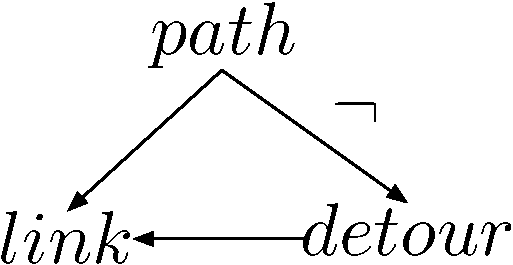
\includegraphics[scale=1]{figures/dependency-graph}
\caption{\label{ch:p2:fig:dependency}Dependency graph for predicates 
appearing in Figure~\ref{ch:p2:fig:negation}.}
\end{center} 
\end{figure*}

Figure~\ref{ch:p2:fig:dependency} contains the dependency graph for the predicates
appearing in the rules of Figure~\ref{ch:p2:fig:negation}. Constructing this graph
is a straightforward application of the following two rules.
\begin{enumerate}
  \ssp
  \item Add $p \rightarrow q$ dependency if there is a rule with head predicate $p$ and subgoal $q$.
  \item Add $p \rightarrow q$ dependency labeled $\neg$ if there is a rule with head predicate $p$ and negated subgoal $q$.
\end{enumerate}
From Figure~\ref{ch:p2:fig:negation}, rule~\ol{R4} forms the $path \rightarrow
link$ and $path \rightarrow detour$ dependencies, while rule~\ol{R5} forms the
$detour {\neg \atop \rightarrow} link$ negated dependency. 

We now formally define the stratum of an IDB predicate to be the largest number
of $\neg$ on a path from that predicate, in the dependency graph. The dependency
graph in Figure~\ref{ch:p2:fig:dependency} places predicates \ol{detour} and \ol{link}
in the lowest stratum~$0$, while the \ol{path} predicate is in stratum~$1$. If all
IDB predicates have a finite stratum, then the Datalog program is stratified. If any
IDB predicate has an infinite stratum, then the program is unstratified. An IDB
predicate is assigned an infinite stratum if it is on a path that contains a cycle 
(due to recursion), and there exists a negated edge along that path. 

We evaluate a stratified Datalog program using the seminaive algorithm of
Figure~\ref{ch:p2:fig:seminaive} but with a slight twist -- we order the
$\delta$-IDB predicates by their assigned stratum.  If the program is
stratified then any negated subgoal (e.g., \ol{detour}) has already had its
relation fully evaluated.  The result of this evaluation is a {\emph stratified
model}. We revisit the notion of stratified Datalog throughout this thesis. It turns
out that the P2 system does not supported stratified Datalog, which significantly
complicated made many of our \OVERLOG programs mentioned in Chapters~\ref{ch:evita}, 
\ref{ch:magic} and~\ref{ch:opt}.


\section{\OVERLOG: The P2 Query Language}
\label{ch:p2:sec:overlog}

\OVERLOG is based on the traditional recursive query language, Datalog.  As in
Datalog, an \OVERLOG~{\em program} consists of a set of deduction {\em rules}
that define the set of tuples that can be derived from a base set of tuples
called {\em facts}.  Each rule has a {\em body} on the right of the \texttt{:-}
divider, and a {\em head} on the left; the head represents tuples that can be
derived from the body.  The body is a comma-separated list of {\em terms}; a
term is either a {\em predicate} (i.e., a relation), a {\em condition} (i.e., a
relational selection) or an {\em assignment}~\footnote{\OVERLOG's assignments
are strictly syntactic replacements of variables with expressions; they are
akin to ``\#define'' macros in C++.}.  An example \OVERLOG program is shown in
Figure~\ref{ch:p2:fig:overlogSP}.  \OVERLOG introduces some notable extensions
to Datalog, which we review before describing the P2 runtime.

\begin{figure*}
\ssp
\begin{boxedminipage}{\linewidth}
{\bf materialize}(link,infinity,infinity,keys(1,2)). \\
{\bf materialize}(path,1,infinity,keys(1,2,3)).  \\
{\bf materialize}(shortestPath,1,infinity,keys(1,2,3)). \\
\\
{\bf link}("localhost:10000", "localhost:10001"). \\
{\bf link}("localhost:10001", "localhost:10002"). \\
\\
R1{\bf path}(@X, Y, P, C) :- \\
\datalogspace {\bf link}(@X, Y, C), P := f\_cons(X, Y). \\
\\       
R2 {\bf path}(@X,Y,P,C) :- \\
\datalogspace {\bf link}(@X, Z, C1), {\bf path}(@Z, Y, P2, C2), \\
\datalogspace $f\_contains(X,P2) == false$, \\
\datalogspace P := f\_cons(X,P2), C := C1 + C2. \\ 
\\      
R4 {\bf minCostPath}(@X, Y, a\_min$<$C$>$) :-  \\
\datalogspace {\bf path}(@X, Y, P, C). \\
\\
R5 {\bf shortestPath}(@X, Y, P, C) :- \\
\datalogspace {\bf minCostPath}(@X, Y, C), {\bf path}(@X, Y, P, C).\\
\end{boxedminipage}
\caption{\label{ch:p2:fig:overlogSP}Shortest path program in \OVERLOG. \ol{a\_}
prefixes introduce aggregate functions and \ol{f\_} prefixes introduce
built-in functions.}
\end{figure*}

\subsection{Horizontal partitioning}

\OVERLOG's basic data model consists of relational tables that are partitioned
across the nodes in a P2 network.  Each relation in an \OVERLOG rule must have
one attribute that is preceded by an ``@'' sign.  This attribute is called the
{\em location specifier} of the relation, and must contain values in the
network's underlying address space (e.g., IP addresses for Internet settings,
802.13.4 addresses for sensor networks, hash-identifiers for code written atop
distributed hash tables, etc.).  Location specifiers define the horizontal
partitioning of the relation: each tuple is stored at the address found in its
location specifier attribute.  At a given node, we call a tuple a {\em local
tuple} if its location specifier is equal to the local address.  Network
communication is implicit in \OVERLOG: tuples must be stored at the address in
their location specifier, and hence the runtime engine has to send some of its
derived tuples across the network to achieve this physical constraint.  Loo, et
al.  provide syntactic tests to ensure that a set of rules can be maintained
partitioned in a manner consistent with its location specifiers and network
topology~\cite{loo-sigmod06}.


\subsection{Soft State and Events}

Associated with each \OVERLOG table is a ``soft-state'' lifetime that
determines how long (in seconds) a tuple in that table remains stored before it
is automatically deleted.  Lifetimes can vary from zero to infinity.
Zero-lifetime tables are referred to as {\em event} tables, and their tuples
are called \emph{events}; all other tables are referred to as {\em
materialized} tables.  \OVERLOG contains a \ol{materialize} declaration that
specifies the lifetime of a materialized table.  At any instant in time, at any
given node in the network, the contents of the local \OVERLOG ``database'' are
considered to be: (a) the local tuples in materialized tables whose lifetime
has not run out, (b) at most one local event fact across {\em all} event
tables, and (c) any derived local tuples that can be deduced from (a) and (b)
via the program rules.  Note that while (b) specifies that only one event fact
is considered to be live at a time per node, (c) could include {\em derived}
local events, which are considered to be live simultaneously with the event
fact.  This three-part definition defines the semantics for a single P2 node at
a snapshot in time.  P2 has no defined semantics across time and space (in the
network); we describe the relevant operational semantics of the prototype in
Section~\ref{sec:eventloop}.
     
\subsection{Deletions and Updates}

\OVERLOG, like SQL, supports declarative expressions that identify tuples to be
deleted in a deferred manner after query execution completes.  To this end, any
\OVERLOG rule in a program can be prefaced by the keyword \ol{delete}.  The
program is run to fixpoint, after which the tuples derived in {\tt delete}
rules -- as well as other tuples derivable from those -- are removed from
materialized tables before another fixpoint is executed.  It is also possible
in \OVERLOG to specify updates, but the syntax for doing so is different.
\OVERLOG's {\tt materialize} statement supports the specification of a primary
key for each relation.  Any derived tuple that matches an existing tuple on the
primary key is intended to {\em replace} that existing tuple, but the
replacement is separated into an insertion and a deletion: the deduction of the
new fact to be inserted is visible within the current fixpoint, whereas the
deletion of the original fact is deferred until after the fixpoint is computed.

\subsection{A Canonical Example}
\label{ch:p2:sec:declnet}

To illustrate the specifics of \OVERLOG, we review the shortest paths example
in Figure~\ref{ch:p2:fig:overlogSP}, which is similar to that
of~\cite{loo-sigmod06}, but with fully-realized \OVERLOG syntax that runs in
P2.  The three \ol{materialize} statements specify that \ol{link}, \ol{path}
and \ol{bestpath} are all tables with infinite lifetime and infinite storage
space\footnote{The third argument of P2's table definition optionally specifies
a constraint on the number of tuples guaranteed to be allowed in the relation.
The P2 runtime replaces tuples in ``full'' tables as needed during execution;
replaced tuples are handled in the same way as tuples displaced due to
primary-key overwrite.}.  For each table, the positions of the primary key
attributes are noted as well.  Rule \ol{r1} can be read as saying ``if there is
a link tuple of the form \ol{(X,Y,C)} stored at node \ol{X}, then one can
derive the existence of a path tuple \ol{(X,Y,P,C)} at node \ol{X}, where
\ol{P} is the output of the function \ol{f\_cons(X,Y)} -- the concatenation of
\ol{X} and \ol{Y}.'' Note that rule \ol{r1} has the same location specifiers
throughout, and involves no communication.  This is not true of the recursive
rule \ol{r2}, which connects any \ol{link} tuple at a node \ol{X} with any path
tuple at a neighboring node \ol{Z}, the output of which is to be stored back at
\ol{X}.  As described in the earlier work on
P2~\cite{loo-sigcomm05,loo-sigmod06} such rules can be easily rewritten so that
the body predicates all have the same location specifier; the only
communication then is shipping the results of the deduction to the head
relation's location specifier.

\section{The P2 Runtime Engine}
\label{ch:p2:sec:p2}

The P2 runtime is a dataflow engine that was based on ideas from relational
databases and network routers; its scheduling and data hand-off closely
resemble the Click extensible router~\cite{click-tocs}.  Like Click, the P2
runtime supports dataflow {\em elements} (or ``operators'') of two sorts:
pull-based elements akin to database iterators~\cite{graefe-survey}, and
push-based elements as well.  As in Click, whenever a pull-based element and a
push-based element need to be connected, an explicit ``glue'' element (either a
pull-to-push driver, or a queue element) serves to bridge the two.  More
details of this dataflow coordination are presented in the original P2
paper~\cite{p2:sosp}.

\subsection{Dataflow Elements} 

The set of elements provided in P2 includes a suite of operators familiar from
relational query engines: selection, projection, and in-memory indexes.  P2
supports joins of two relations in a manner similar to the symmetric hash join:
it takes an arriving tuple from one relation, inserts it into an in-memory
table for that relation, and probes for matches in an access method over the
other relation (either an index or a scan).  The work described in
Chapter~\ref{ch:evita} extended this suite to include sorting and merge-joins,
which allowed us to explore some traditional query optimization opportunities
and trade-offs (Section~\ref{ch:evita:sec:systemr}).

P2 currently has no support for persistent storage, beyond the ability to read
input streams from comma-separated-value files.  Its tables are stored in
memory-based balanced trees that are instantiated at program startup;
additional such trees are constructed by the planner as secondary indexes to
support query predicates.

P2 also provides a number of elements used for networking, which handle issues
like packet fragmentation and assembly, congestion control, multiplexing and
demultiplexing, and so on; these are composable in ways that are of interest to
network protocol designers~\cite{condie-hotnets05}.  The basic pattern that the
reader should assume is that each P2 node has a single IP port for
communication, and the dataflow graph is ``wrapped'' in elements that handle
network ingress with translation of packets into tuples, and network egress
with translation of tuples into packets.

\subsection{The P2 Event Loop}
\label{sec:eventloop}

The control flow in the P2 runtime is driven by a fairly traditional event loop
that responds to any network or timer event by invoking an appropriate dataflow
segment to handle the event.

The basic control loop in P2 works as follows:
\begin{CompactEnumerate}
    \item An event is taken from the system input queue, corresponding to a single newly-arrived tuple, which is either an {\em insert} tuple (i.e., the result of a normal deduction) or a {\em delete} tuple (the result of a \ol{delete} rule or a primary-key update).  We will refer to this tuple as the {\em current tuple}.
    \item The value of the system clock is noted in a variable we will call the {\em current time}.  This is the time that will be used to determine the liveness of soft-state tuples.  
    %(Note that any event tuples that arrived previously will no longer be live in any event table, which guarantees the single-event semantics described above.)
    \item The current tuple is, logically, appended to its table.
    \item If the current tuple is an insert tuple, the dataflow corresponding to the \OVERLOG program is initiated and run to a local fixpoint following traditional Datalog semantics, with the following exception: during processing, any non-local derived tuples are buffered in a {\em send queue}, as are any derived tuples to be deleted.
    \item If, instead, the current tuple is a delete tuple, the dataflow
    is run to a local fixpoint, but newly-derived local tuples
    (including the current tuple) are copied to a {\em delete queue},
    and newly-derived non-local tuples are marked as delete tuples
    before being placed in the send queue so as to cascade the deletions
    to remote nodes' databases.
    \item All tuples in the delete queue are deleted from their associated tables, and the delete queue is emptied.
    \item The send queue is flushed across the network, with any local updates inserted into the local input queue.
\end{CompactEnumerate}

Unlike Datalog, \OVERLOG must run in the continuous processing context of
networking, over streams of tuples representing system events.  This inherently
requires more than the single computation of a fixpoint as described in the
Datalog literature.  P2 has modified its handling of this issue since the
initial paper~\cite{p2:sosp}.  P2 nests a fairly traditional declarative
Datalog fixpoint execution within an operationally defined local event loop at
each node.  An input queue is kept at each P2 node, to hold tuples that
correspond to network messages and clock interrupts.  Each tuple in the queue
is tagged with the name of a relation in the schema of the Datalog database.
The loop begins by noting the local wall-clock time, and deleting from all
tables any tuples whose soft-state lifetime has expired; this includes event
tuples from the previous iteration of the loop.  At that point, a tuple is
dequeued from the input queue and inserted into its associated table.  At that
point, the \OVERLOG program is run to fixpoint atomically, nearly as if it were
a traditional single Datalog program.  One exception to traditional Datalog is
the handling of derived tuples with remote location specifiers; these are
placed directly into network queues for subsequent processing.  Another
exception involves rules that have {\em actions} in the head -- these actions
can be table insertion or deletion; derived tuples in such rules are also
enqueued for subsequent processing.  When fixpoint is reached, the queued
network messages are sent to their destinations, and the table actions are
carried out on the database.  This completes one iteration of the event loop.

From this perspective, the P2 runtime looks quite a bit like an
Event-Condition-Action system with dataflow underneath: events are provided by
the clock and network, conditions are checked via the dataflow engine for
matches, which are then converted into actions: network messages to be sent, or
table updates to be performed.

\section{Summary}

While ostensibly a network protocol engine, architecturally P2 resembles a
fairly traditional shared-nothing parallel query processor, targeted at both
stored state and data streams.  The P2 runtime at each node consists of a
compiler---which parses programs, optimizes them, and physically plans them---a
dataflow executor, and access methods.  Each P2 node runs the same query
engine, and, by default, participates equally in every ``query.'' In parallel
programming terms, P2 encourages a Single-Program-Multiple-Data (SPMD) style
for parallel tasks, but also supports more loosely-coupled (MPMD) styles for
cooperative distributed tasks, e.g.  for communications among clients and
servers.


% \jmh{This is probably too long.  Also, we need to purge text that was recycled from SOSP.  }
% The design of P2 was inspired by prior work in both databases and
% networking. It is based in large part upon a
% side-by-side comparison between the PIER peer-to-peer query
% engine~\cite{pier-cidr05} and the Click router~\cite{click-tocs}. Like
% PIER, P2 can manage structureddata tuples flowing through a broad
% range of query processing elements, which may accumulate significant
% state and perform substantial asynchronous processing.  Like Click, P2
% stresses high-performance transfers of data units, as well as dataflow
% elements with both ``push'' and ``pull'' modalities. 
% 
% At a coarse grain, P2 in its current state consists of (1) an \OVERLOG
% parser, (2) an Planner that translates \OVERLOG to a runtime dataflow
% plan, and (3) a runtime plan executor.  The
% life of a query is simple: the query is parsed into an internal
% representation, the planner constructs a corresponding dataflow graph
% of elements, and the graph is executed by the runtime until it is
% canceled.  We proceed to overview the components bottom-up; more
% details are given in the P2 SOSP paper~\cite{p2:sosp}.
% 
% Processing in P2 is handled with a dataflow model inspired by Click
% and PIER.  As in Click, nodes in a P2 dataflow
% graph can be chosen from a set of C++ objects called
% \textit{elements}.  In database systems these are often called
% \textit{operators}, since they derive from logical operators in the
% relational algebra.  Elements have some number of input and output
% \emph{ports}.  An arc in the dataflow graph is represented by a
% binding between an output port on one element and an input port on
% another.  Tuples arrive at the element on input ports, and elements
% emit tuples from their output ports. Handoff of a tuple between two elements takes one
% of two forms, \emph{push} or \emph{pull}, determined when the elements
% are configured into a dataflow graph.   
% 
% P2 provides a number of built in dataflow elements that allow it to
% implement networking and query processing logic.  This includes
% elements for the streaming relational query operators found in most
% database systems, e.g., selection, projection, join, and aggregation.
% It also includes networking elements responsible for socket handling,
% packet scheduling, congestion control, reliable transmission, data
% serialization, and dispatch.  P2 has elements to store incoming tuples in tables, 
% iteratively emit tuples in a table matching a filter expression, and {\em listener}
% elements that are notified whenever a tuple is added or deleted from a
% table. Finally, like Click, P2 includes a collection of general-purpose
% ``glue'' elements, such as a queue, a multiplexer, a round-robin
% scheduler, etc.
% 
% Storage in P2 is currently via a main-memory relational Table
% implementation, named using unique IDs that can be shared between
% different queries and/or dataflow elements.  In-memory indices
% (implemented using standard balanced binary trees) can be attached to
% attributes of tables to enable quick equality lookups.  The current
% in-memory implementation serves the system requirements for implementing
% network overlays and streaming query applications, all of which tend
% to expire tuples from memory rather than accumulating them
% indefinitely.  P2's event-driven, run-to-completion model obviates the
% need for locking or transaction support, and relatively simple indices
% suffice to meet performance requirements.  We plan additional
% table implementations that use stable storage for persistent data
% storage; that engineering task is relatively straightforward, but not
% within the scope of this paper.
% 

\section{Clustering and Classification}
\label{cc} 
We use affinity propagation \cite{ap} for clustering spammers that have the same sending behavior. We discuss the clustering and classification techniques applied to our system in Section~\ref{cluster} and Section~\ref{classify}. Section~\ref{ap} gives an explanation of affinity propagation. 

\subsection{Clustering}
\label{cluster} 
Our clustering and classification phase is similar to SpamTracker \cite{bb}. Spammers are clustered only on their sending behavior, which is determined by finding the domains a spammer targets. Email contents are not taken into consideration. To gather data concerning a spammer's sending behavior, we collect data for over two hundred distinct email domains. 
\begin{equation}
       \displaystyle M \leftarrow \sum_{k = 1}^t M'(i, j, k)
       \label{eq:collapse}
\end{equation}

In the clustering phase, we generate a matrix $M$ \emph{n}x\emph{d}, where \emph{n} is the number of IP addresses that sent emails to \emph{d} domains in a time interval \emph{t}. A period of 6 hours is used to gather the number of messages that an IP sends to the \emph{d} domains in that time interval. 

In order to get the similarity matrix $S$ \emph{n}x\emph{n}, which is used in the affinity propagation algorithm, the dot product between two IP addresses is calculated. When
calculating the similarity that data point \emph{i} shares with data point \emph{j}, the dot product is normalized. 
\begin{equation}
	\displaystyle S(i, j) \leftarrow \frac{M(i, j) \bullet M(i, j)'}{\sum_{k=1}^d M(j,k)}
	\label{eq:similarity}
\end{equation}

The clusters generated in the clustering phase do not have common IP addresses between them. Each cluster represents a spammer traffic pattern. The cluster center is computed by averaging the traffic pattern of the IP addresses present in the cluster. The cluster average is a \emph{1}x\emph{d} vector.
\begin{equation}
	\displaystyle c_{avg}(j) \leftarrow \frac{\sum_{i=1}^{\vert C \vert} M_c(i,j)}{\vert C \vert}
	\label{eq:cavg}
\end{equation}

\subsection{Classification}
\label{classify} 
In the classification phase, the sending pattern of an IP address \emph{T}, a \emph{1}x\emph{d} vector, is determined, and then a score is calculated to determine the similarity of its traffic pattern with one of the clusters. This score is the maximum of the normalized dot product between the sending pattern of the IP address being tested and the set of cluster averages found in Equation~\ref{eq:cavg}. 
\begin{equation}
	\displaystyle Score \leftarrow \max_{C} \frac{T(1, j) \bullet c_{avg}(i, j)'}{\sum_{j=1}^d c_{avg}(i,j)'}
	\label{eq:score}
\end{equation}
\\

Since we are attempting to determine the sending patterns of spammers across multiple domains, we ignore clusters that are dominated by a single domain. Also, spammers that target a single domain will tend to give scores of one to benign, non-spamming, IP addresses since non-spamming IP addresses will tend to send emails to a single domain in a short duration. 

A single round of classification involves classifying the set of IP addresses, that send email within the next six hour period using the set of clusters found in the preceding time interval. 

\subsection{Affinity Propagation}
\label{ap} 
Affinity propagation is a message passing algorithm that clusters similar data points. The algorithm sends messages between each variable in the algorithm. In a naive distributed implementation, each variable can be a node in the network, which sends messages across the network edges until a set of exemplars and their corresponding clusters have been found. An exemplar is a variable that lies in the center of the cluster.

The algorithm takes as input a similarity matrix $S$ of $n$x$n$ size for $n$ data points. $S(i,j)$ represents the similarity data point \emph{i} has with data point \emph{j}. The similarity matrix does not need to be symmetric, that is the similarity data point \emph{j} has with data point \emph{i} does not need to be the same as data point \emph{i}'s similarity with data point \emph{j}. Data point \emph{k}'s similarity with itself is referred to as the preference for data point \emph{k} as its own exemplar. Preferences with large values are more likely to be chosen as an exemplar. The initial preference values  determines the number of clusters. If each data point is just as likely to be an exemplar, preferences should all be set to a common value. For our experiments, the preferences were set to the median similarity of a given IP address. 

There are two kind of messages that are sent between data points. The \emph{responsibility message r(i,k)} represents how well suited data point \emph{k} is as the exemplar of \emph{i}.
\begin{equation}
	\displaystyle r(i,k)\leftarrow s(i,k)-\max_{k' s.t. k' \neq k}\{a(i,k') + s(i,k')\}
	\label{eq:resp}
\end{equation}

Availability messages are sent from candidate exemplar \emph{k} to data point \emph{i} suggesting whether \emph{k} will be a good exemplar for \emph{i}.
\begin{eqnarray*}
	\displaystyle a(i,k) \leftarrow \min\{0,r(k,k) + \\
    \sum_{i' s.t. i' \notin \{i,k\}}\max\{0, r(i',k)\}\}	
    \label{eq:avail}
\end{eqnarray*}
\begin{equation}
\end{equation}
Self-availability is updated using:
\begin{equation}
	\displaystyle a(k,k) \leftarrow \sum_{i' s.t. i' \neq k} \max\{0, r(i',k)\}
	\label{eq:self}
\end{equation}

At any point in time, exemplar for data point \emph{i} can be found by combining the responsibilities and availabilities.
\begin{equation}
	\displaystyle exemplar(i) \leftarrow \argmax_{k} \{a(i,k) + r(i, k)\}
	\label{eq:exemplar}
\end{equation}

Data points that have no similarity (a similarity of zero in our experiments) do not need to send messages between them. If data points do not share any similarity, these points should never be exemplars for each other. The availabilities and responsibilities are constantly updated in an iterative process: responsibilities are first updated given the availabilities (these are initially set to zero), availabilities are updated given the newly calculated responsibilities, and finally the exemplars for each iteration are calculated. 

Once the exemplars have converged, the affinity propagation algorithm terminates. As responsibilities and availabilities for each data point are updated, oscillations can occur. To prevent oscillations, we use a damping factor, $\lambda$, with a value between 0 and 1 whereby each message is set to $\lambda$ times it previous value plus 1 minus $\lambda$ times its new value. 

\section{Architecture}
\label{sec:arch}
In this section, we present a strawman design that incorporates our
defenses and particular design choices from Section~\ref{sec:defenses}.
We first describe the randomness oracle, specify how peers validate node
identifiers usi
We first present the components involved and then the updated protocols
for overlay maintenance.

\subsection{Components}
In our strawman design, in addition to regular peers, there is a
distinguished component providing
identifier unpredictability, the \emph{randomness oracle}.  The
determination of peer identifiers is performed by peers based on input
from the randomness oracle.


\subsection{Randomness Oracle}
\label{sec:epoch_server}
The state of a randomness oracle consists of its history of chosen
random numbers, along with the times at which those numbers were
assigned.  The oracle forgets random numbers far enough in the past that
no current peer identifier is computed from them. \comm{Varun}{Should we explain
why 2*$G$ and not just $G$} Typically, this means
remembering no more than $2 \times G$ random number certificates; for
256 churn groups this means about 75 KBytes of total state, which can
conceivably be accommodated even in the CPU cache of a low-end PC-based
server. Note that randomness certificates have a short lifetime (on the
order of minutes), so a revocation mechanism is not required.

Certificates are issued once per time-step.  Even for time-steps on the
order of a few seconds, the required processing is no more than the cost
of signing a new certificate (16 bits for the time-step number, 160 bits
for the random number), which can well-be accommodated by a low-end CPU.

In our simple design, a peer who is about to change identifiers obtains
the appropriate randomness certificates from the oracle.  It can forward
those certificates to peers with which it interacts
while moving to a new position in the overlay; those peers need not
contact the oracle for those certificates and can easily cache them
until expiration. As an optimization, the randomness oracle could
conceivably IP-multicast a stream of randomness certificates to all peers
in the overlay; a newcomer peer first joins the multicast group and then
starts the process of joining the overlay, with a time overhead of no more
than a few
network round trip times.


\subsection{Peer Links}
\label{sec:links}
\comm{Varun}{We dont need to store Randomness certis in the RT once
we have verified their authenticity. Only storing the expiration time should do?
Storing the random certificate for each entry gives the feeling of a castro 
approach}
\comm{Tyson}{Yes we do: if I get a routing table entry from you then I will
want the certificate that tells me its ok. }

Entries in a peer's routing table or leaf set have the form 
\{\emph{NodeID}, \emph{IP Address}, \emph{Expiration Time-step},
\emph{Randomness Certificate}\}.  The included randomness certificate
corresponds to the time-step at which the referent of the entry changed
identifiers; the expiration time-step is there primarily for
convenience, and to prepare for future designs in which 
identifiers have different lifetimes.

\comm{Varun}{such=? Non referential such?}
A correct peer can verify the compliance of such entries as follows.
\begin{enumerate}
\item Compute the churn group to which the entry IP address belongs.
\item Verify that the randomness certificate corresponds to that churn
  group.
\item Verify that the randomness certificate has not expired, i.e.,
  the churn group has not churned again since this certificate was
  issued. In our simple scheme, this means checking that $t \geq
  T_\mathit{now} - 2kG$.   comm{Sriram}{An explanation of what t and Tnow are. And saying that the 2 accounts for stale certificates etc.}

\item Verify the signature of the certificate (no need to check for
  revocation). \comm{Varun}{We could combine this step with step 2?}
\item Verify the mapping from IP address and randomness certificate to
  node identifier.\comm{Varun}{Could we put this more simpler as: verify
  nodeID=SHA1(nodeIP||randomness certificate)}
\end{enumerate}
This verification need only be performed once for each entry, until the
associated identity expires.



\subsection{Routing Table Maintenance}
\label{sec:routing_state}
When a peer joins a logical area of the network, it provides a reference
to itself, in the form described in Section~\ref{sec:links}, to peers
that wish to add it to their routing tables or leaf sets.
Before a peer inserts such an entry into its routing state, it validates
the entry by itself, and then ensures that no diversity rules are
violated; if either check fails, the entry is rejected.  In our simple
design, the only diversity rule we use is that no more than $d$ entries
in a peer's routing table and leaf set may have the same unspoofable
identifier.
Periodically (no faster than every $k$ time-steps), a peer cleans out
entries from its routing state that have expired.

Peers maintain two sets of routing state, one set for high-performance
routing that incorporates optimizations such as proximity neighbor
selection, and one \emph{constrained} set, formed as described by Castro
et al.~\cite{Castro2002short}.  The constrained routing state is used to
precompute routing state across identifier changes.\comm{Sriram}{An explanation of what t and Tnow are. And saying that the 2 accounts for stale certificates etc.}


Soon before it has to change identifiers, a peer precomputes the 
\emph{prospective} constrained routing table and leaf set, corresponding
to its next
node identifier.  It starts computing this prospective routing state
immediately after it receives the random number at its next churn
time-step (either via multicast, or by contacting the randomness
oracle).  The peer obtains its prospective leaf set by routing to its
next node identifier a request for the leaf set of the node currently
there.  It obtains its prospective routing table entries, again,  in a fashion similar to the
formation of the constrained routing table described by Castro et
al.~\cite{Castro2002short}, as well as the discovery algorithm in
Bamboo~\cite{Rhea2004short}.  Specifically, for an entry in the $r$-th
row and $c$-th column of the prospective routing table, the peer routes
a lookup request to the nearest occupant of the node identifier with the
same $r$ high-order digits, $c$ as its $r+1$-st digit, and a locally
selected random number for its low-order digits. Entries for both the
prospective leaf set and the routing table are dropped if they are due
to expire before the peer will have moved to its new logical position. 
All lookups for the precomputation of prospective routing state are
routed over the current constrained routing table.

To change identifiers, a peer announces its impending arrival to its
prospective leaf set and switches routing state, initializing both
current routing state sets with the prospecting routing state it
precomputed.  For specific application, this is also the time when the
peer might off-load any keys it currently stores (e.g., in a DHT
scenario).  Note that if the prospective leaf set contains no valid
(i.e., correct and unexpired) entries, then the peer is forced to
completely rejoin the network anew.



\section{Evaluation models}

Consider the \emph{successor} relation described above.  According to our intuitive interpretation, this relation models
the passage of time, in order to establish a temporal order among ground atoms.  More formally, we expect of a successor
relation that

$\forall A,B (successor(A, B) \rightarrow B > A) \land \forall A \exists B (successor(A, B))$

This implies that successor is infinite (as we'd expect time to be), and is problematic because it leads to unsafe programs.

\newtheorem{example}{Example}
\begin{example}
Consider the program and EDB below.

\begin{Dedalus}
r1
p_pos(A, B)@next \(\leftarrow\)
  p_pos(A, B),
  \(\lnot\)p_neg(A, B);
  
p_pos(A, B)  \(\leftarrow\)
  p(A, B);
  
p(1, 2)@123;
  
\end{Dedalus}

The single ground fact will, due to \emph{r1}, cause as many deductions as there are tuples in the \emph{successor} relation.
Clearly, if the relation is infinite this program in unsafe.

\end{example}

But if \emph{successor} is infinite, many of these are in some sense \emph{void deductions}, functionally determined based on the EDB.
In effect,  and EDB that is given in its totality determines a window over successor that is relevant to any computation that must be performed.  
It is easy to see that in this example, we need only consider a successor relation that contains a single tuple \{123, 124\}.

Consider the given EDB extended with two more facts:

\begin{Dedalus}
delete p(1, 2)@456;
p(?, ?)@789;
\end{Dedalus}

Evaluating this program and EDB will require a \emph{successor} relation with values that range from 123 - 789.

\begin{definition}
A \emph{post-hoc} evaluation is an evaluation of a Dedalus program in which an EDB is given, \emph{successor} is derived from it
as part of a fixpoint computation.
\end{definition}

In a post-hoc evaluation, we may use the given EDB to populate the successor relation in the following way.
Define first a second order predicate called \emph{event\_time} 
that contains the union of the time attributes from the EDB prefix. Let \emph{Trace} be the set of $n$ EDB predicates.  
Then \emph{event\_time} is defined as

$event\_time(\Tau) \leftarrow \displaystyle\bigcup_{i}^n \pi_{\Tau}Trace_{i}$

We populate \emph{successor} with a negation-free Datalog program with arithmetic and aggregate functions, as shown below.

\begin{Dedalus}
smax(max<N>) \(\leftarrow\) event\_time(N);
smin(min<N>) \(\leftarrow\) event\_time(N);

successor(N, N + 1) \(\leftarrow\) smin(N);

successor(S, S + 1) \(\leftarrow\) 
    successor(N, S),
    smax(M),
    N <= M;
\end{Dedalus}

In a post-hoc evaluation, time is in some sense ``instantaneous" in that all values of the successor relation are considered in a single
fixpoint computation.  The complete program is safe if the EDB is finite.

\subsection{EDB Prefixes}
\paa{notes follow}

In general, an EDB can itself be infinite. 

\begin{definition}
A \emph{prefix} $\alpha_{n}$ of an EDB $\Gamma$ is the set of events whose timestamp is greater than or equal to $n$.
\end{definition}

If the EDB is finite, then it has a maximum timestamp $\top$, and $\alpha_{\top}$ = $\Gamma$.  Because each prefix is strictly larger than
all prefixes with lower indices, we also have:

$\forall \alpha_{i}, \alpha_{j} \in \Gamma ((i < j) \to (\alpha_{i} \subset \alpha_{j}))$.

Consider a function $FP$ from $Program, EDB \mapsto IDB$ that represents the \emph{fixpoint} computation carried out by a datalog interpreter.
We would like to show that 

$FP(P, \alpha_{k}) =  \displaystyle \bigcup_{i=0}^{k} FP(P, \alpha_{i})$ for any $k$.  

this could (with some work) lead to an inductive proof
that an infinite model is minimal.  we could prove the (weaker?) property that
the infinite series of models of increasing finite prefixes of an EDB are all 
minimal if one of them is.

below is just a sketch of a proof:

\begin{proof}

Inductive step:

if we assume that some program P and finite prefix $\alpha_n$ of a trace $\Gamma$ produce a minimal model, 
then it follows that a prefix $\alpha_{n+1}$ and the IDB produced by the previous model produce a minimal model.

Assume the contrary: there is some program P, prefix $\alpha_i$ and prefix $\alpha_j$  s.t. $\alpha_j$ follows $\alpha_i$, $I_1$ = FP($\alpha_i$) is a minimal model 
and $I_2$ = FP($\alpha_j \cup I_1$) is not.  

then in $I_2$ there exists a ground atom that is not in $\alpha_j$ (and hence not in $\alpha_i$), and is not entailed by P given $\alpha_j$.  
such a ground atom must then either be:

\begin{enumerate}
\item contained in $I_1$, hence entailed by P given $\alpha_i$.
\item entailed by P given some IDB atom in $I_1$.
\end{enumerate}

In the first case, in principle is it possible for an atom X to exist in $I_1$ and not in $I_2$, if for example it depended negatively via a 
rule r on a predicate q, and a q fact (Y) exists in  $\alpha_j$ that didn't exist in  $\alpha_i$.  However, for this to occur, because a ground atom 
in I1 cannot depend upon a ground atom from the "future", that event q would need to have occurred at some time less than 
or equal to the to timestamp of atom X.  but this is not possible, because our trace is ordered in timestamp order.  hence the 
first case leads to contradiction.

in the second case, there is some ground atom Y in I1 upon which X depends.  Y is not in FP( $\alpha_j$), because if it were, X would 
be part of the single minimal model.  if Y is not in FP( $\alpha_j$), it too is not part of a minimal model for P given  $\alpha_j$!  if it is in the minimal 
model for FP($\alpha_i$) but not FP( $\alpha_j$), there must be a fact in  $\alpha_j$ upon which an atom in FP($\alpha_i$) depended negatively.  by the same 
argument as above, such a fact could not be in  $\alpha_j$, because new facts in  $\alpha_j$ have timestamps strictly higher than those in  $\alpha_i$.
\end{proof}

Even without providing a basis, we may say
\section{Related Work}
\label{related}
Content-based or IP-based blacklisting techniques are traditional approaches used for spam filtering. Content-based filtering techniques evaluate the content of the message to classify spams. The techniques tend to either use Bayesian filtering techniques to classify email as spam \cite{bayesian,spambayes,sahami98bayesian} or use a signature or checksum \cite{dcc} of the message to compare it against a spam database on the Internet. Both these techniques require training data that captures the contents in the spam. Moreover, spammers dynamically add textual polymorphism to their spam to evade such filters.

Blacklists (\cite{spamhaus,spamcop,uribl,dnsbl}) contain IP addresses that are considered to be associated with spammers. Many spam filters (\cite{spamassassin,mailavenger}) use these lists along with other content-based schemes. These lists can be static or dynamic and are stored in databases that can be queried \cite{dnsbl}. Reactive blacklists try to update the list based on tracking whether an IP address is associated with a spammer and update the list as the IP addresses are altered (\cite{spamhaus,spamcop,uribl}).

Pure content-based filtering techniques have become ineffective because spammers change email content frequently by using images in the email, or by sending well crafted emails that affect the Bayesian learner or classifier~\cite{wittel-wu-2004-attacking, nelson-etal-2008-spambayes}. IP-address based blacklists work for fixed IP addresses, but become outdated quickly, requiring the need to be updated frequently. These issues have led to detecting spam based on an IP address' sending or traffic pattern \cite{bb,Spamhints}. Ramachandran et al. proposes that spammers do not change their sending pattern frequently, thus making it efficient to detect them based on their sending behavior~\cite{bb}. The sending behavior of a spammer is determined by the frequency of emails sent by the spammer to each domain. Similar concept has been used in SpamHINTS \cite{Spamhints,clayton04stopping,DBLP:conf/ceas/Clayton05}. SpamHINTS uses heuristics related to \emph{Simple Mail Transfer Protocol} (SMTP) sessions of a sender. These include measuring delivery failures and analyzing delivery failure messages. It has been suggested that blacklisting spammers based on their sending behavior can be complemented with other traditional techniques to provide better spam detection.

It is difficult to detect coordinated spamming attacks by botnets because spammers keep their local activity below threshold.  Characterization studies \cite{sb} have observed that the local view of malicious spamming activity remains undetected due to the low volume of activity. This raises the need to aggregate spammers' activity across domains. A popular approach uses clustering to identify groups of spam messages or hosts. Li et al. cluster spammers based on the URL present in the emails and find huge clusters of spammers having the same URL \cite{cluster1}. The method proposed by Anderson et al. identifies cluster of web servers that host graphically similar websites linked from the messages \cite{spamscatter}. The graphic similarity between websites is found using a technique called \emph{image shingling}. This method is used to find web servers hosting phishing websites. Both of these methods use email contents for clustering. Clustering was also used to identify spammers based on their sending pattern as computed by SpamTracker \cite{bb}.

Most of the approaches discussed above \cite{bb,cluster1,spamscatter} are centralized and exhibit disadvantages such as scalability and single point of failure.  The schemes established by Damiani et al. and Alex and Dmitry Brodsky outline a system that collaboratively shares information to detect spammers \cite{sabrina04ppbased,trinity} . Damiani et al. propose comparing incoming messages to known spam messages classified by an automatic mechanism or by final recipients \cite{sabrina04ppbased}. Techniques like message digests, URLs in the email and originating mail servers can be used for comparison. Alex Dmitry Brodsky present an approach that counts the quantity of emails to determine whether the emails were sent from spamming bots \cite{trinity}.

\section{Conclusion and Future Work}

\jmh{In here, please follow up on the intro -- discuss how we built some serious shit in Overlog, and we believe that \lang is just 
as expressive because its operational semantics (cite boom-tr) are essentially the same as the behavior of Algorithm 1.  Formalizing this
a bit difficult since it entails developing a proper definition of the operational semantics of our Overlog interpreter.  Rather than trouble ourselves
with that, we are in the process of ``porting'' our Overlog code to Dedalus. }
Datalog has inspired a variety of recent applied work, which touts the benefits of declarative specifications for practical implementations.  Unfortunately, Datalog's declarative semantics make no guarantees
regarding the order in which derivations will occur; or rather, they derive all derivations in one atomic fixpoint computation.  This makes it difficult to associate natural ``side-effects'' like state update and message delivery with purely logical notions of deduction.


\lang is the result of our experience using hybrid
declarative/imperative languages such as Overlog~\cite{Loo2009-CACM}
to implement a number of networking protocols and distributed
systems~\cite{boom-techr,Alvaro2009I-Do-Declare:-C,Chu:2007,Loo2009-CACM}.
Although our experience with those languages was largely positive, the
combination of Datalog and imperative constructs hampered our
development of program analyses, and even our understanding of the
``correct'' execution of single-node programs that performed state
updates.

By mapping time to another type of data over which logical deductions
are performed, \lang allows us to express concepts such as asynchrony and state update in terms of a purely deductive logic
language, achieving the goal of a declarative language without sacrificing critically expressive features for the distributed systems domain.

\jmh{I think this paragraph says ``\lang handles state'', and the next says ``\lang handles asynchrony.''  Yes?  Let's say so than.}
At their core, state update and communication differ from logical
deductions only in terms of timing; \lang's notion of time allows us
to interleave operations and time in terms of logical deductions.
In the local case, this allows us to express state update without giving up the clean semantics of Datalog; unlike
Datalog extensions that use imperative constructs to provide such
functionality, each \lang rule expresses a logical invariant that will
hold over all program executions.  
\jmh{next sentence is lost of me.}
Our treatment of time in terms of
logical constraints allows us to model issues such as causality (and
``clever'' systems that observe causality violations) in a flexible
manner.

However, interactions with external processes, and primitives such as
asynchronous and unreliable communication introduce nondeterminism
which \lang models with \dedalus{choose}.  

Our hope is that modeling external process and events with a single
primitive will greatly simplify program analysis techniques.  Rather
than spending time and effort translating imperative code into sets of logical
invariants over program executions, analyses of \lang programs can
work directly against the invariants encoded by the program, allowing
them to focus on invocations of \dedalus{choose}, each of which
encodes some less easily avoided source of non-determinism and
ambiguity, such as a hardware failure or end-user.

\rcs{not really happy with the last paragraph; we should at least say some high-level thing about raising level of abstraction of programming, enabling more applications, etc, etc...}

\section{Conclusion}
\label{concl}
In this paper, we proposed using P2 to implement a distributed version of affinity propagation for detecting spammers. P2 allows us to easily develop a distributed approach to spam filtering using declarative programming, which keeps our program concise. This distributed implementation allows domain-mail servers to classify emails in real-time, and works as well as the centralized spectral clustering algorithm used by SpamTracker \cite{bb}. 
\section{Acknowledgment}
We thank Prof. Nick Feamster and Anirudh Ramachandran for providing the SpamTracker dataset and giving insight into their design and algorithms, as well as Prof. Joe Hellerstein and Prof. Vern Paxson for their directions and comments.

\bibliographystyle{plain}
\small{\bibliography{paper}}

\appendix
\section{Appendix}
\label{appendix}
\definecolor{myblue}{rgb}{0.8,0.85,1}

\begin{tabular}{|l|}
\hline
\rowcolor{myblue} Materialized relations \\
\hline
\scriptsize{\textit{/*node, Var, CandidateExemplar, value*/}} \\
\scriptsize{materialize(availability, infinity, infinity, keys(2,3)).} \\

\scriptsize{\textit{/*node, LocalVar, CandidateExemplar, value*/}} \\
\scriptsize{materialize(responsibility, infinity, infinity, keys(2,3)).} \\

\scriptsize{\textit{/*node, LocalVar, CandidateExemplar, value*/}} \\
\scriptsize{materialize(sentResponsibility, infinity, infinity, keys(2,3)).} \\

\scriptsize{\textit{/*node, LocalVar, CandidateExemplar, value*/}}\\
\scriptsize{materialize(similarity, infinity, infinity, keys(2,3)).} \\

\scriptsize{\textit{/* node, Var, CandidateExemplar, max(Responsibility, 0)*/}} \\
\scriptsize{materialize(rp, infinity, infinity, keys(2,3)).} \\
\hline
\end{tabular}


\begin{tabular}{|l|}
\hline
\rowcolor{myblue} Update responsibilities for each iteration\\
\scriptsize{\textit{/*Responsibility updates for each local variable}}\\
\scriptsize{\textit{at a periodic time interval*/}}\\
\scriptsize{rUpdate(@N, LocalVar) :-}\\
\scriptsize{ \hspace{0.5cm}        periodic(@N,E, AP\_EPOCH),}\\
\scriptsize{ \hspace{0.5cm}        localVariable(@N, LocalVar, \_).}\\
        
\scriptsize{\textit{/*Ordered set of similarity + availability (AS)}}\\
\scriptsize{\textit{The customized a\_Max2Details aggregate function}}\\
\scriptsize{\textit{returns the ordered pair of (candidate exemplars, AS)}}\\
\scriptsize{\textit{with the largest two AS values*/}}\\
\scriptsize{asSet(@N, LocalVar, a\_Max2Details\textless{}AS\textgreater{}) :- }\\
\scriptsize{ \hspace{0.5cm}        rUpdate(@N, LocalVar),}\\
\scriptsize{ \hspace{0.5cm}        availability(@N, LocalVar, CE, A,),}\\
\scriptsize{ \hspace{0.5cm}        similarity(@N, LocalVar, CE, S),}\\
\scriptsize{ \hspace{0.5cm}        AS := A + S.}\\


\scriptsize{\textit{/*Responsibility calcuations for a given r(i,k)}}\\
\scriptsize{\textit{i can be considered the LocalVar and k is the variable CE}}\\
\scriptsize{\textit{The CE here only relates to the candidate exemplars that}}\\
\scriptsize{\textit{do not produce the maximum AS value for the LocalVar, i}}\\
\scriptsize{\textit{This is detailed in \textbf{Equation 3.5*/}}}\\
\scriptsize{responsibilityEvent(@N, LocalVar, CE, NR) :-}\\
\scriptsize{ \hspace{0.5cm}        asSet(@N, LocalVar, Max2Details),}\\
\scriptsize{ \hspace{0.5cm}        similarity(@N, LocalVar, CE, S), }\\
\scriptsize{ \hspace{0.5cm}        MaxAS := f\_removeLast(Max2Details),}\\
\scriptsize{ \hspace{0.5cm}        MaxCE := f\_removeLast(Max2Details),}\\
\scriptsize{ \hspace{0.5cm}        NR := Similarity - MaxAS,}\\
\scriptsize{ \hspace{0.5cm}        CE != MaxCE.}\\

\scriptsize{\textit{/*Responsibility calcuations for a given r(i,k)}}\\
\scriptsize{\textit{i can be considered the LocalVar and k is the variable CE}}\\
\scriptsize{\textit{The CE here only relates to the candidate exemplars that}}\\
\scriptsize{\textit{does produce the maximum AS value for the LocalVar, i}}\\
\scriptsize{\textit{This is detailed in \textbf{Equation 3.5}*/}}\\
\scriptsize{responsibilityEvent(@N, LocalVar, CE, NR)  :-}\\
\scriptsize{ \hspace{0.5cm}        asSet(@N, LocalVar, Max2Details),}\\
\scriptsize{ \hspace{0.5cm}        similarity(@N, LocalVar, CE, S),}\\
\scriptsize{ \hspace{0.5cm}        MaxAS := f\_removeLast(Max2Details),}\\
\scriptsize{ \hspace{0.5cm}        MaxCE := f\_removeLast(Max2Details),}\\
\scriptsize{ \hspace{0.5cm}        MaxAS2 := f\_removeLast(Max2Details),}\\
\scriptsize{ \hspace{0.5cm}        MaxCE2 := f\_removeLast(Max2Details),}\\
\scriptsize{ \hspace{0.5cm}        NR := S - MaxAS2,}\\
\scriptsize{ \hspace{0.5cm}        CE == MaxCE.}\\

\scriptsize{\textit{/*This rules sends the responsibilities across the network}}\\
\scriptsize{\textit{the variable relation contains the location (IP address/port)}}\\
\scriptsize{\textit{of the candidate exemplar (CE)*/}}\\
\scriptsize{responsibility(@CEN, LocalVar, CE, R)  :-}\\
\scriptsize{ \hspace{0.5cm}        responsibilityEvent(@N, LocalVar, CE, NR)}\\
\scriptsize{ \hspace{0.5cm}        variable(@N, CE, CEN).}\\
        
\scriptsize{sentResponsibility(@N, LocalVar, CE, R)  :-}\\
\scriptsize{ \hspace{0.5cm}        responsibilityEvent(@Node, LocalVar, CE, R).}\\
\hline
\end{tabular}\\

\begin{tabular}{|l|}
\hline
\rowcolor{myblue} Update availabilities for each iteration\\
\hline
\scriptsize{\textit{/*Availabilitiy updates for each local variable}}\\
\scriptsize{\textit{at a periodic time interval*/}}\\
\scriptsize{aUpdate(@Node, CE, Var) :-}\\
\scriptsize{ \hspace{0.5cm}         periodic(@N, E, AP\_EPOCH),}\\
\scriptsize{ \hspace{0.5cm}         localVariable(@N, CE, \_),}\\
\scriptsize{ \hspace{0.5cm}         similarity(@N, CE, Var, \_).}\\

\scriptsize{\textit{/* The summation in \textbf{Equation 3.6}*/}}\\        
\scriptsize{sumRp(@N, Var, CE, a\_SUM\textless{}RP\textgreater{}) :-}\\
\scriptsize{ \hspace{0.5cm}         aUpdate(@N, CE, Var),}\\
\scriptsize{ \hspace{0.5cm}         rp(@N, OtherVar, CE, RP),}\\
\scriptsize{ \hspace{0.5cm}         OtherVar != Var,}\\
\scriptsize{ \hspace{0.5cm}         OtherVar != CE.}\\

\scriptsize{\textit{/*Availability calculations \textbf{Equations 3.6}*/}}\\
\scriptsize{availabilityCalc(@N, Var, CE, NA) :-}\\
\scriptsize{ \hspace{0.5cm}         sumRp(@N, Var, CE, SumRP),}\\
\scriptsize{ \hspace{0.5cm}         responsibility(@N, CE, CE, R),}\\
\scriptsize{ \hspace{0.5cm}         A := SumRP + R,}\\
\scriptsize{ \hspace{0.5cm}         NA := f\_min(A, 0.0),}\\
\scriptsize{ \hspace{0.5cm}         Var != CE.}\\

\scriptsize{\textit{/*Self-availability calculations \textbf{Equations 3.7}*/}}\\
\scriptsize{availabilityCalc(@N, CE, CE, NA) :-}\\
\scriptsize{ \hspace{0.5cm}        sumRp(@N, Var, CE, SumRP),}\\
\scriptsize{ \hspace{0.5cm}         NA := SumRP}\\
\scriptsize{ \hspace{0.5cm}         Var == CE.}\\

\scriptsize{\textit{/*This rules sends the availabilities across the network}}\\
\scriptsize{\textit{the variable relation contains the location (IP address/port)}}\\
\scriptsize{\textit{of the Var variable*/}}\\
\scriptsize{availability(@VarNode, Var, CE, NA)  :-}\\
\scriptsize{ \hspace{0.5cm}         availabilityCalc(@N, Var, CE, NA)}\\
\scriptsize{ \hspace{0.5cm}         variable(@Node, Var, VarNode).}\\
\hline
\end{tabular}
\newpage
\begin{tabular}{|l|}
\hline
\rowcolor{myblue} Exemplar calculation\\
\hline
\scriptsize{\textit{/*Exemplar updates for each local variable}}\\
\scriptsize{\textit{at a periodic time interval*/}}\\
\scriptsize{eUpdate(@N, LocalVar) :-}\\
\scriptsize{ \hspace{0.5cm}        periodic(@N, E, AP\_EPOCH),}\\
\scriptsize{ \hspace{0.5cm}         localVariable(@N, LocalVar, \_).}\\

\scriptsize{\textit{/*Exemplar calculations from \textbf{Equation 3.8}*/}}\\
\scriptsize{exemplarCalc(@N, LocalVar, a\_MAX\textless{}Sum\textgreater{}) :- }\\
\scriptsize{ \hspace{0.5cm}         eUpdate(@N, LocalVar),}\\
\scriptsize{ \hspace{0.5cm}         availability(@N, LocalVar, CE, A),}\\
\scriptsize{ \hspace{0.5cm}         sentResponsibility(@N, LocalVar, CE, R),}\\
\scriptsize{ \hspace{0.5cm}         Sum := A + R.}\\

\scriptsize{exemplar(@N, LocalVar, CE) :-}\\
\scriptsize{ \hspace{0.5cm}         exemplarCalc(@N, LocalVar, MaxSum),}\\
\scriptsize{ \hspace{0.5cm}         availability(@N, LocalVar, CE, A),}\\
\scriptsize{ \hspace{0.5cm}         sentResponsibility(@N, LocalVar, CE, R),}\\
\scriptsize{ \hspace{0.5cm}         MaxSum == A + R.}\\
\hline
\end{tabular}

\end{document}
